\chapter{Manual de usuario}
\label{anexo:manual_usuario}

Este anexo describe el uso básico de Harmony Hub desde el punto de vista de una
persona usuaria final.

\section{Requisitos previos}
\label{sec:manual_usuario_requisitos}

Para utilizar la aplicación se necesita:

\begin{itemize}
    \item un dispositivo Android con la aplicación instalada;
    \item conexión a Internet;
    \item una cuenta de usuario autenticable en la app;
    \item una cuenta de Spotify para generar playlists reales;
    \item permiso de micrófono únicamente si se quiere analizar el entorno.
\end{itemize}

No es necesario conceder acceso al micrófono para completar el flujo principal,
ya que el análisis del entorno es opcional.

\section{Instalación o acceso}
\label{sec:manual_usuario_instalacion}

En el entregable actual, la aplicación se encuentra instalada en un dispositivo
Android físico. El acceso para la persona usuaria consiste simplemente en abrir
la app, iniciar sesión y trabajar con ella desde el móvil.

Para que el flujo completo funcione con generación de playlists reales, el
backend debe estar activo en la infraestructura de demostración y accesible
desde la misma red que el dispositivo. Esta dependencia no afecta al uso normal
de la interfaz, pero sí a la creación de playlists y al cierre completo del
ciclo con Spotify.

Una vez abierta la app, el flujo inicial es:

\begin{enumerate}
    \item iniciar sesión o registrarse;
    \item acceder a la pantalla principal;
    \item conectar la cuenta de Spotify cuando la app lo solicite;
    \item volver al inicio para comenzar un check-in.
\end{enumerate}

\subsection*{Recorrido recomendado de uso}

Para entender la aplicación de forma ordenada, el recorrido recomendado es el
siguiente:

\begin{enumerate}
    \item \textbf{Acceso y autenticación.} Abrir la app, iniciar sesión o crear
    una cuenta nueva.
    \item \textbf{Conexión con Spotify.} Autorizar la cuenta externa para poder
    crear playlists reales al final del flujo.
    \item \textbf{Entrada al check-in.} Volver a la portada y pulsar
    \textit{Empezar check-in}.
    \item \textbf{Definición del contexto.} Responder al objetivo de la sesión,
    estado emocional, energía, estrés y preferencias musicales.
    \item \textbf{Medición opcional del entorno.} Activar, si se desea, el
    análisis del ambiente para enriquecer la recomendación.
    \item \textbf{Revisión de la recomendación.} Leer la explicación funcional
    del modo sugerido y comprobar cómo se adapta al momento actual.
    \item \textbf{Generación de playlist.} Crear la playlist final y abrirla en
    Spotify para escucharla.
    \item \textbf{Cierre con feedback.} Indicar si la sesión ha resultado útil
    para alimentar el aprendizaje posterior del sistema.
\end{enumerate}

Las capturas incluidas en este anexo siguen precisamente ese orden, de forma
que puedan leerse como una guía visual del uso real de Harmony Hub.

\begin{figure}[htbp]
    \centering
    \begin{minipage}{0.31\textwidth}
        \centering
        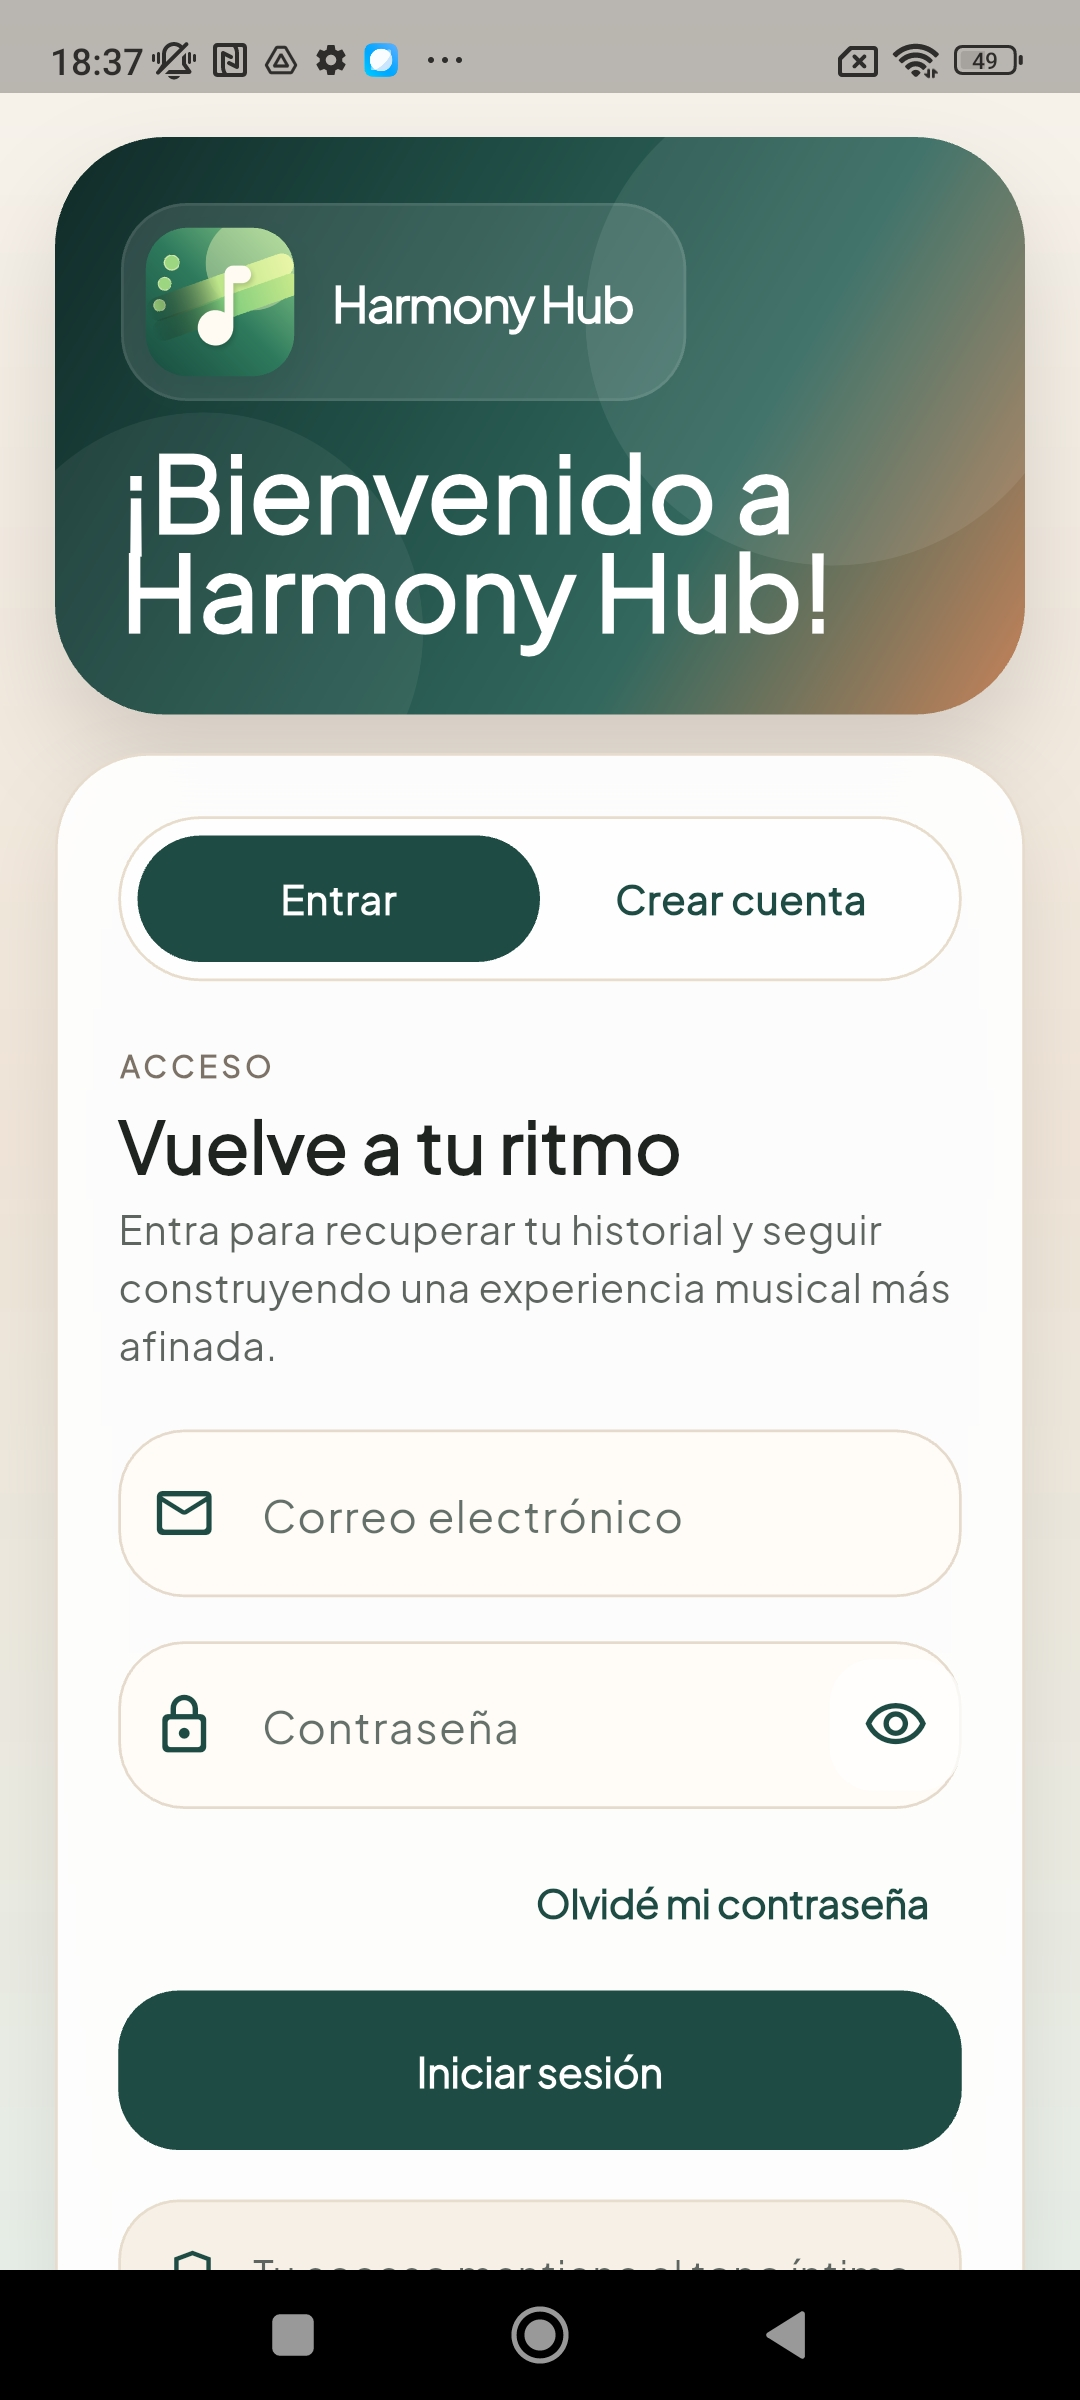
\includegraphics[width=\linewidth]{Imagenes/manual_app/Screenshot_2026-05-25-18-37-08-051_com.example.harmonyhub.jpg}
    \end{minipage}
    \hfill
    \begin{minipage}{0.31\textwidth}
        \centering
        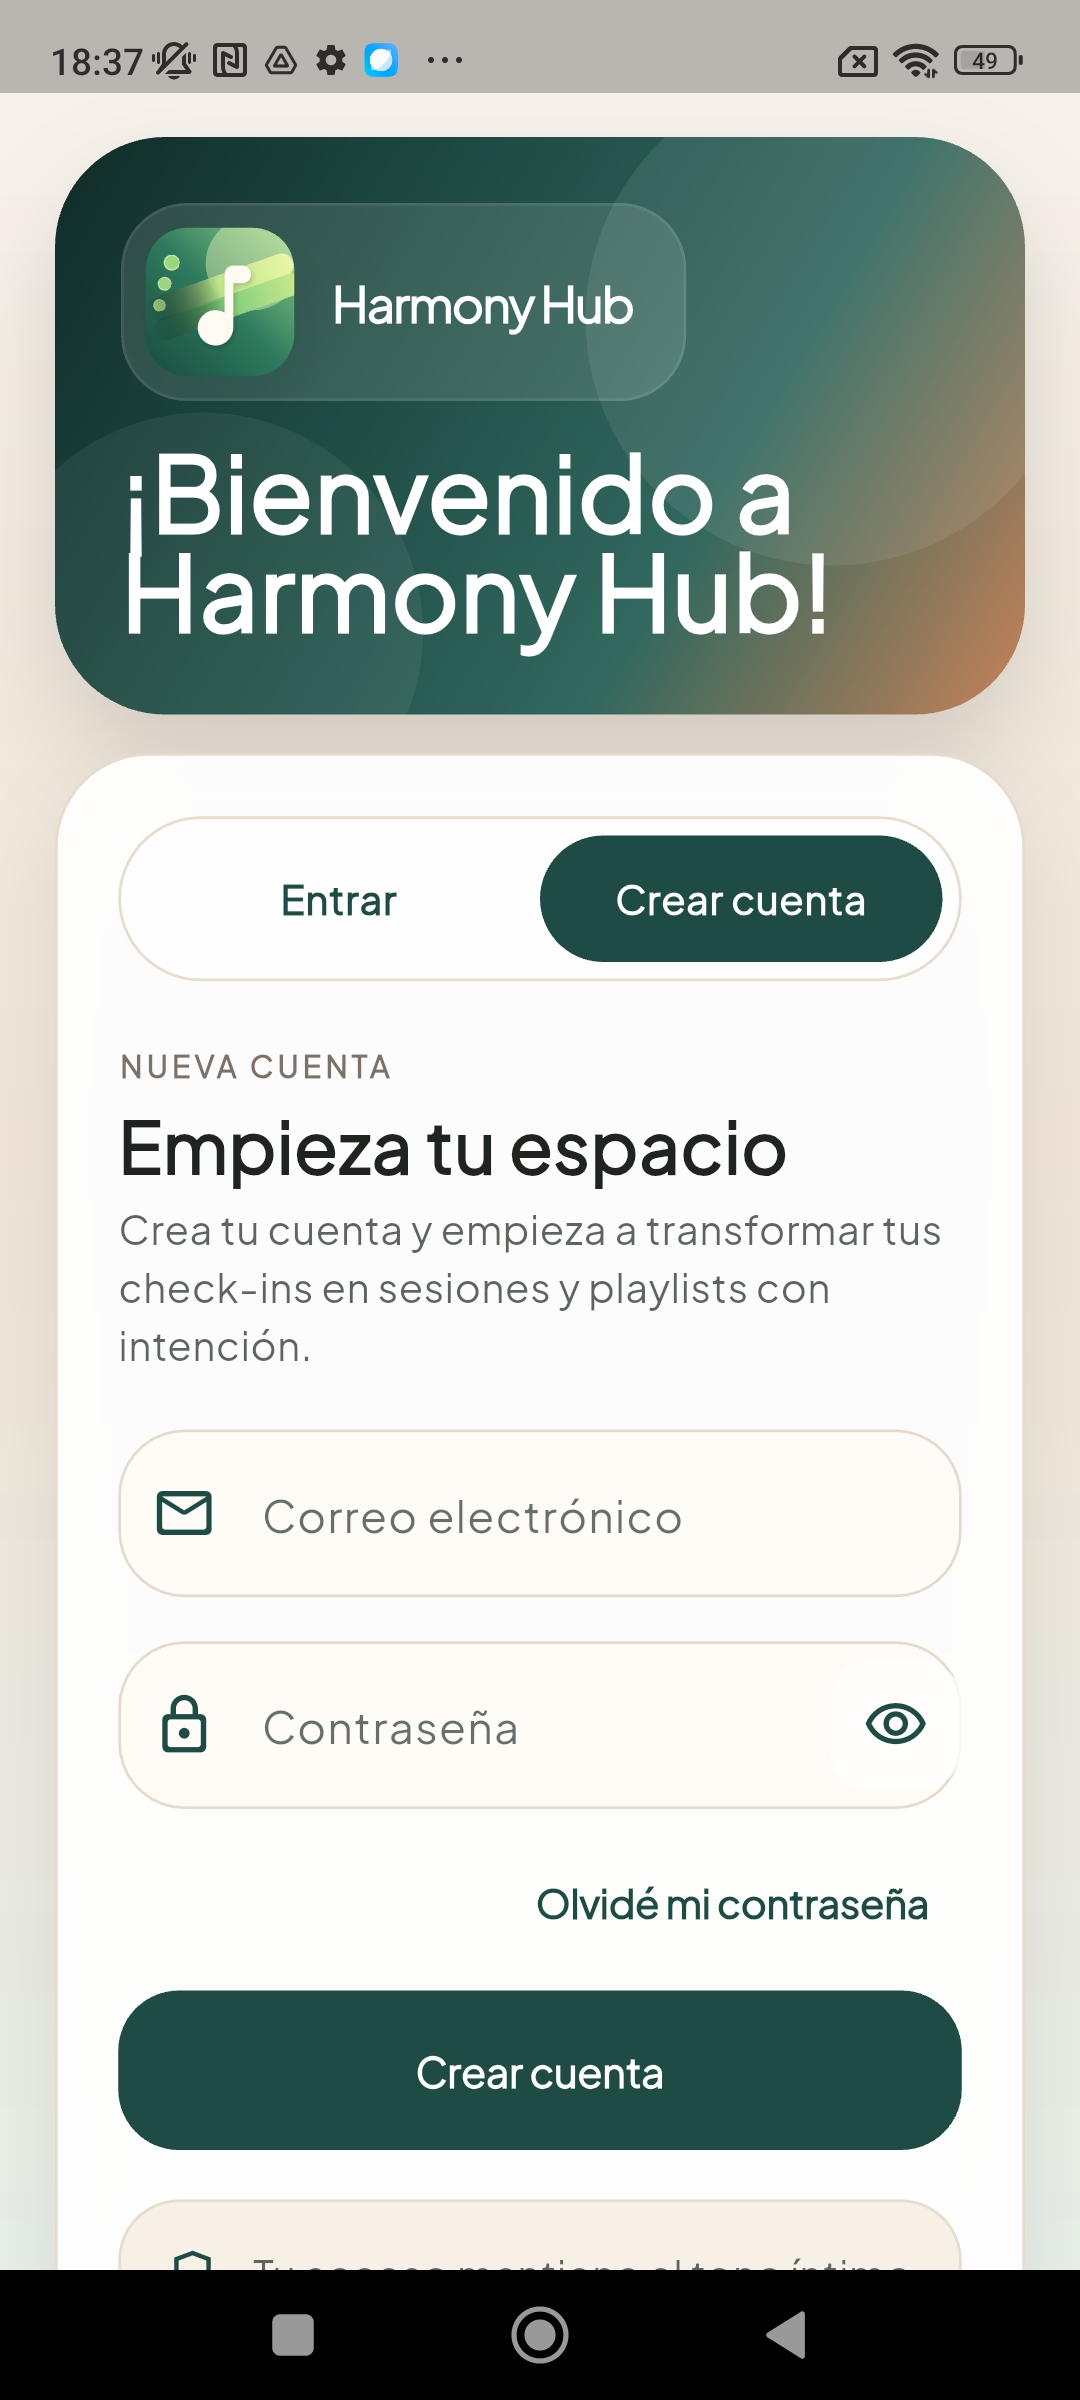
\includegraphics[width=\linewidth]{Imagenes/manual_app/Screenshot_2026-05-25-18-37-25-565_com.example.harmonyhub.jpg}
    \end{minipage}
    \hfill
    \begin{minipage}{0.31\textwidth}
        \centering
        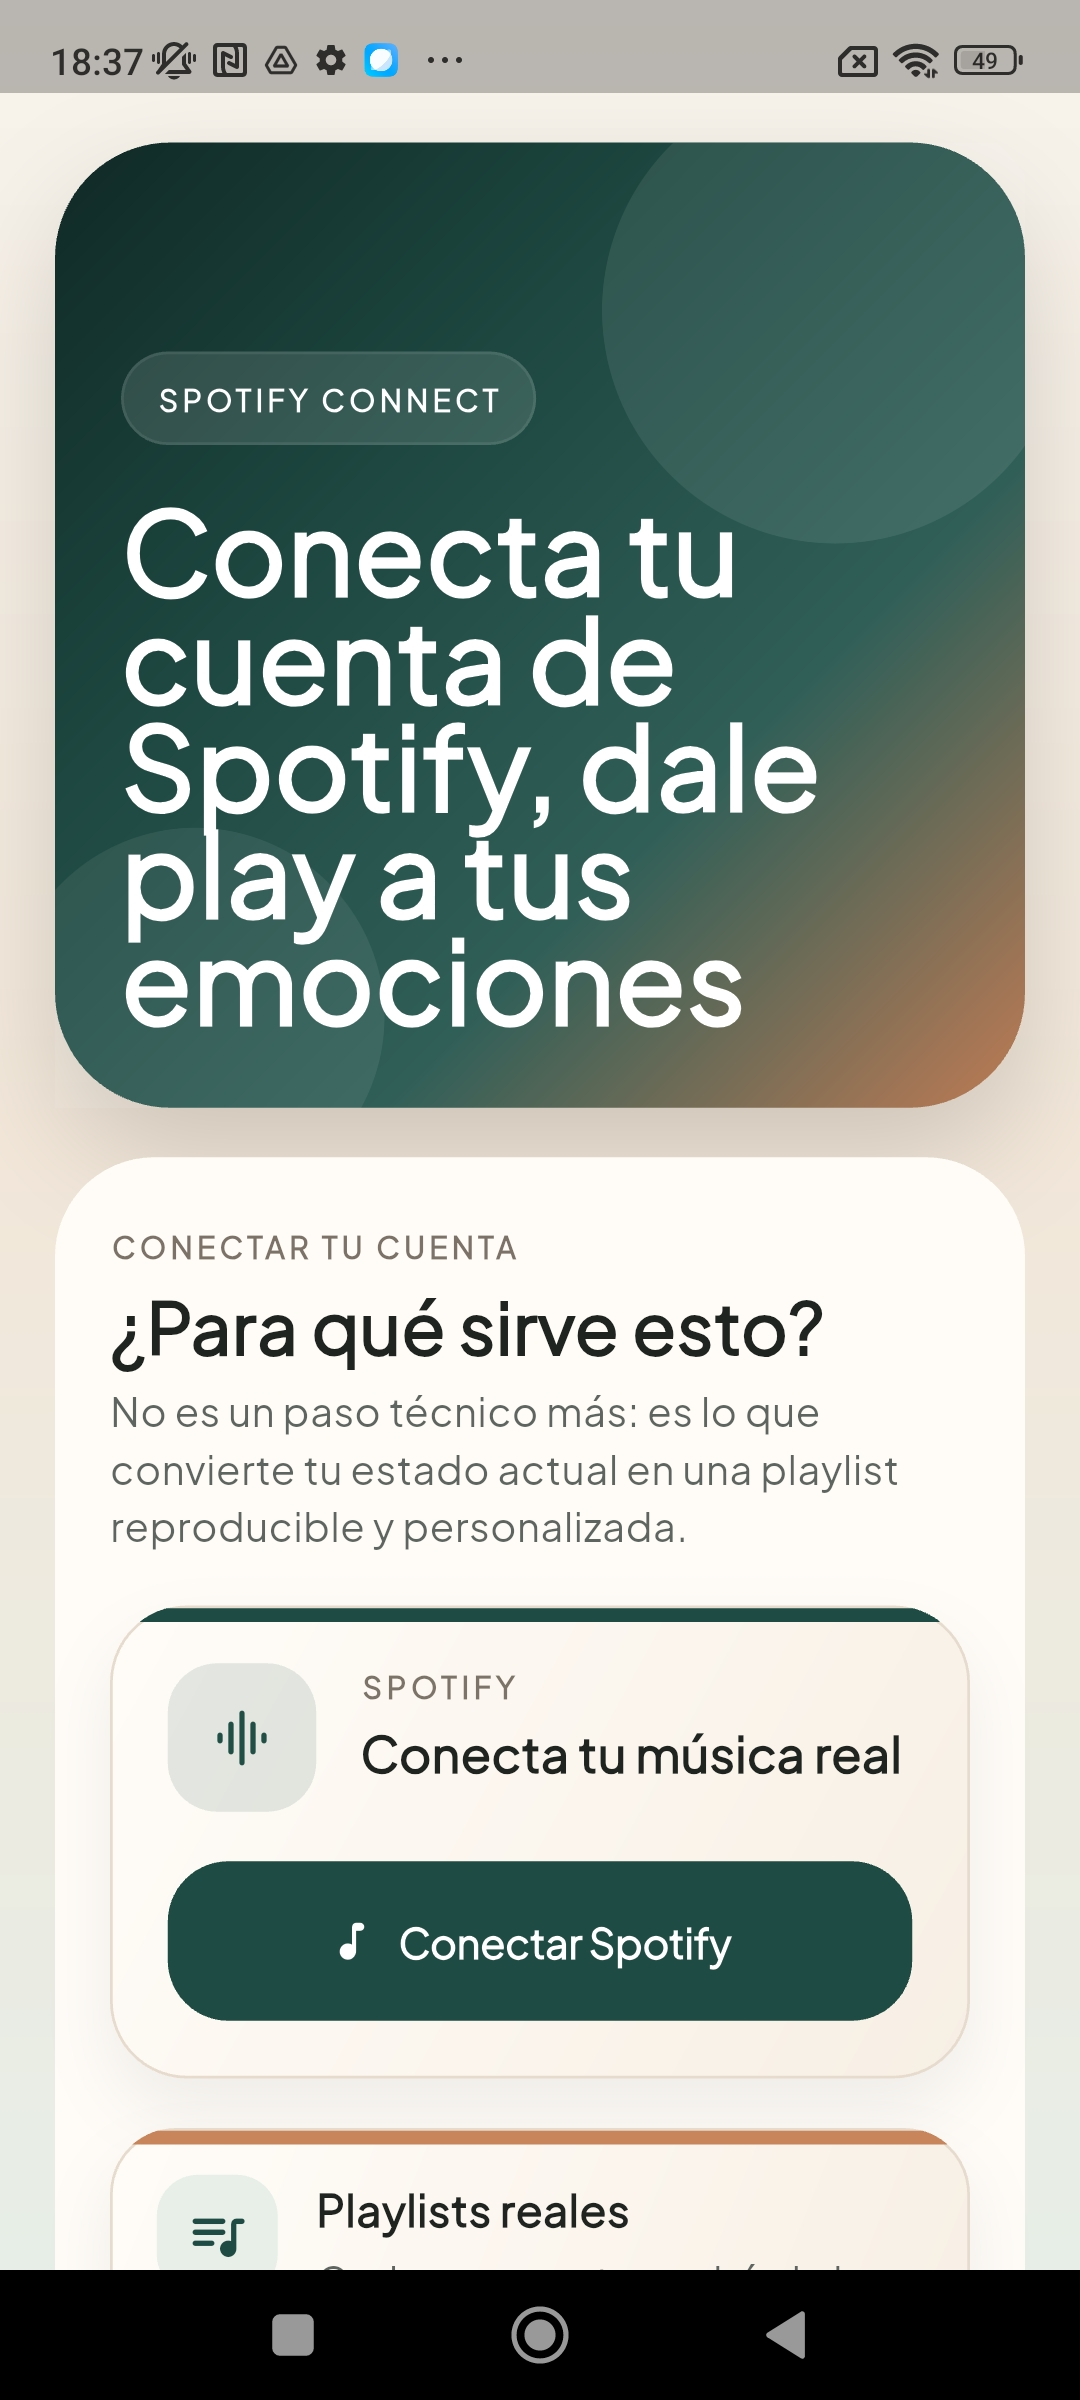
\includegraphics[width=\linewidth]{Imagenes/manual_app/Screenshot_2026-05-25-18-37-46-036_com.example.harmonyhub.jpg}
    \end{minipage}
    \caption{Pantallas iniciales del flujo de acceso: bienvenida e inicio de
    sesión, creación de cuenta y conexión obligatoria con Spotify antes de
    generar playlists reales.}
    \label{fig:manual_acceso_spotify}
\end{figure}

La figura~\ref{fig:manual_acceso_spotify} muestra el primer tramo del flujo de
uso. Primero aparece la pantalla de acceso, desde la que es posible iniciar
sesión o registrar una cuenta nueva. Una vez autenticada la persona usuaria, la
app solicita la conexión con Spotify, ya que esta integración es la que permite
materializar la recomendación final como playlist reproducible.

\section{Uso básico}
\label{sec:manual_usuario_uso_basico}

El flujo de uso normal puede resumirse en seis pasos:

\begin{enumerate}
    \item \textbf{Iniciar un check-in.} El usuario accede a la pantalla de
    check-in y responde preguntas breves sobre su momento actual.
    \item \textbf{Indicar el objetivo de la sesión.} Puede elegir, por ejemplo,
    foco, relajación o energía.
    \item \textbf{Ajustar preferencias.} La app permite indicar intensidad,
    preferencia vocal, nivel de exploración, popularidad deseada y resultado
    esperado.
    \item \textbf{Analizar el entorno si se desea.} Opcionalmente puede medir
    el contexto acústico del momento.
    \item \textbf{Generar la recomendación.} La aplicación muestra la sesión
    sugerida y, si el usuario la acepta, permite crear la playlist real.
    \item \textbf{Cerrar con feedback.} Tras escuchar la playlist, el usuario
    puede valorar si le resultó útil y cómo terminó la sesión.
\end{enumerate}

\subsection*{Pantalla principal y acceso al check-in}

\begin{figure}[htbp]
    \centering
    \begin{minipage}{0.47\textwidth}
        \centering
        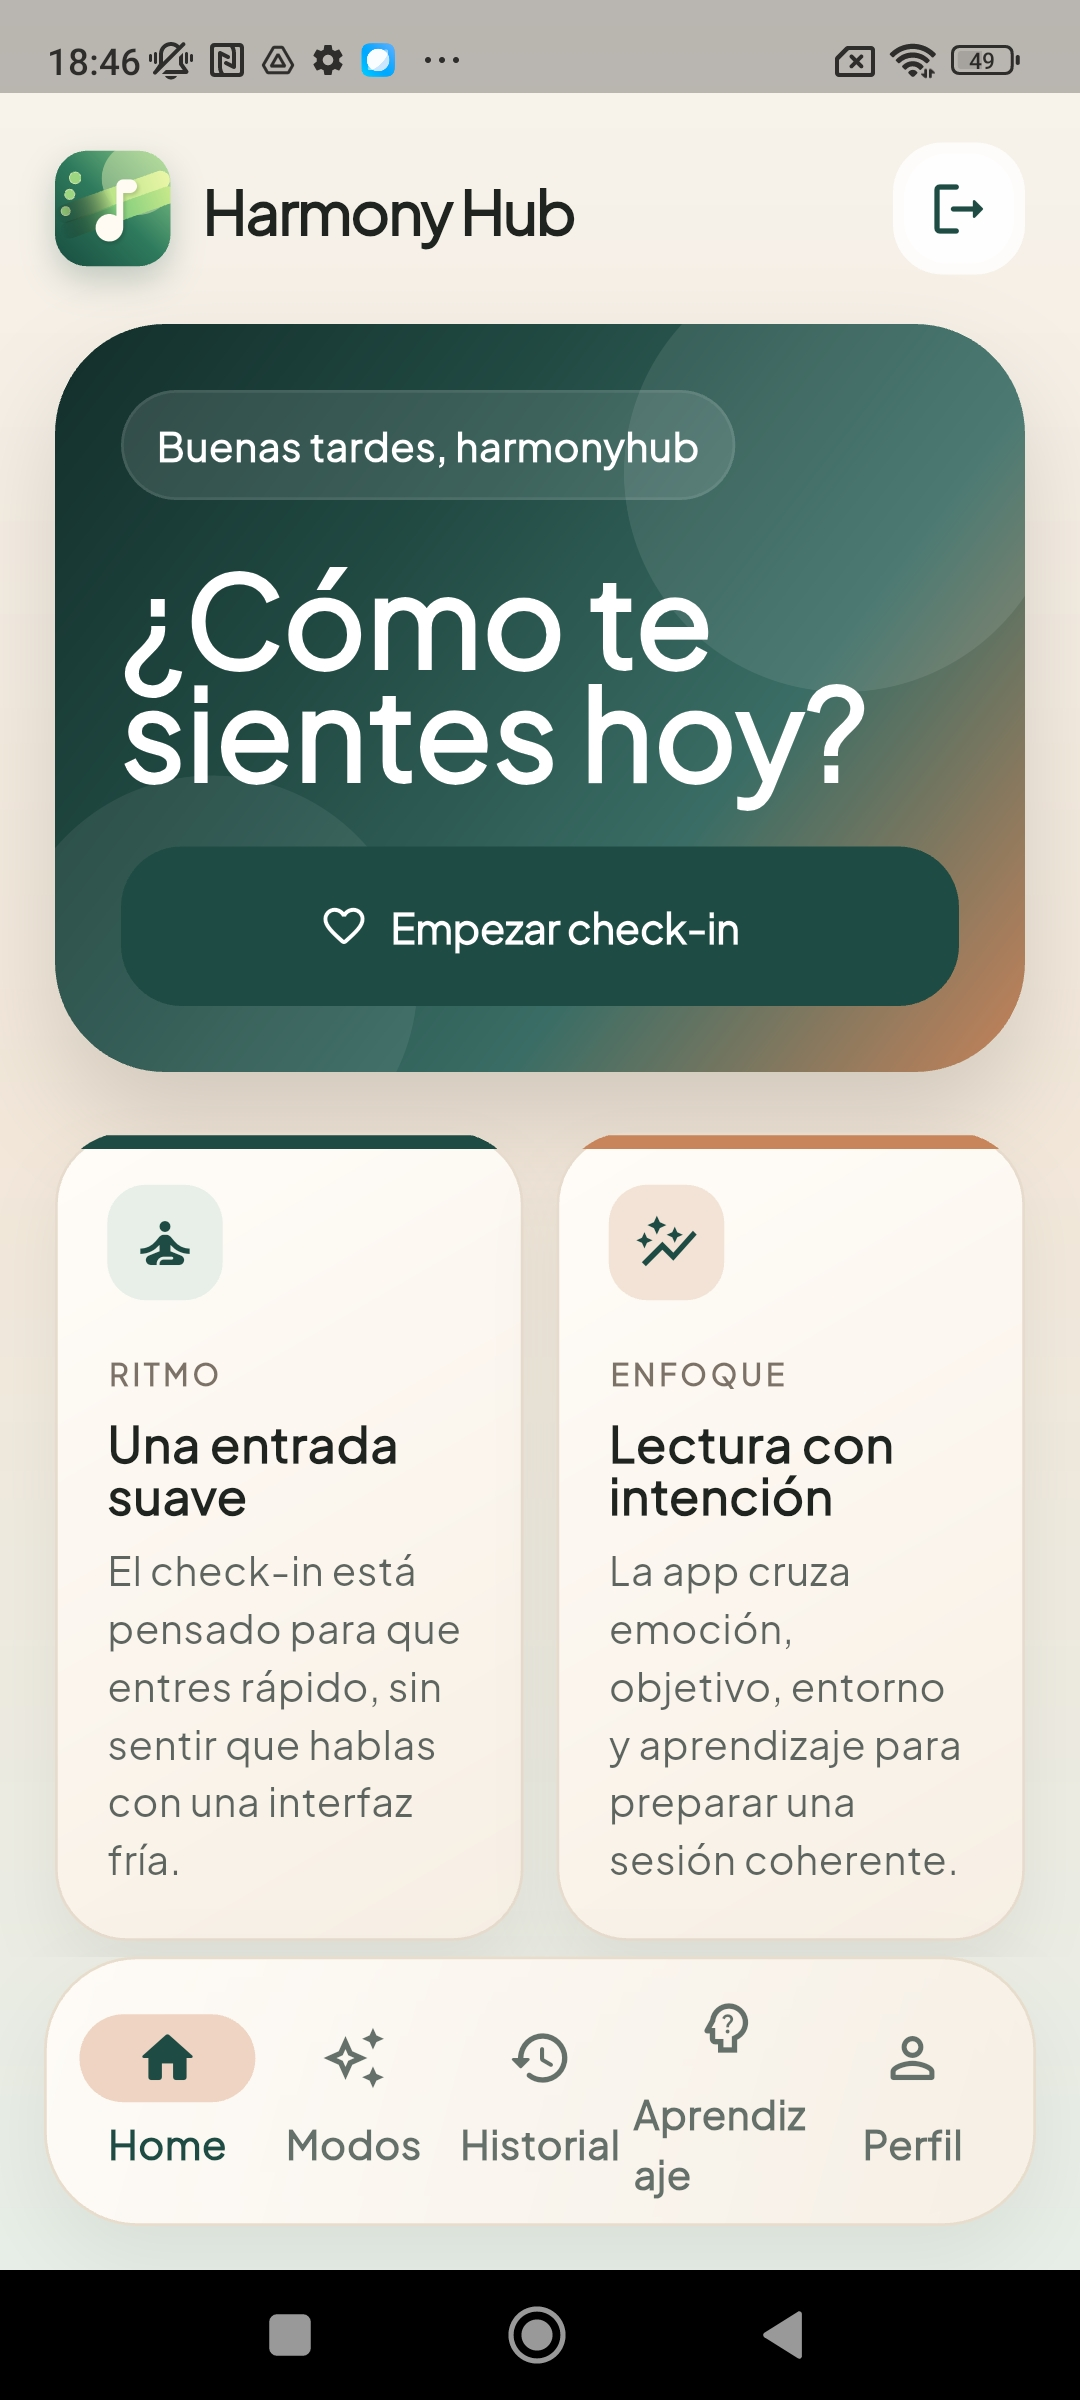
\includegraphics[width=\linewidth]{Imagenes/manual_app/Screenshot_2026-05-25-18-46-14-698_com.example.harmonyhub.jpg}
    \end{minipage}
    \hfill
    \begin{minipage}{0.47\textwidth}
        \centering
        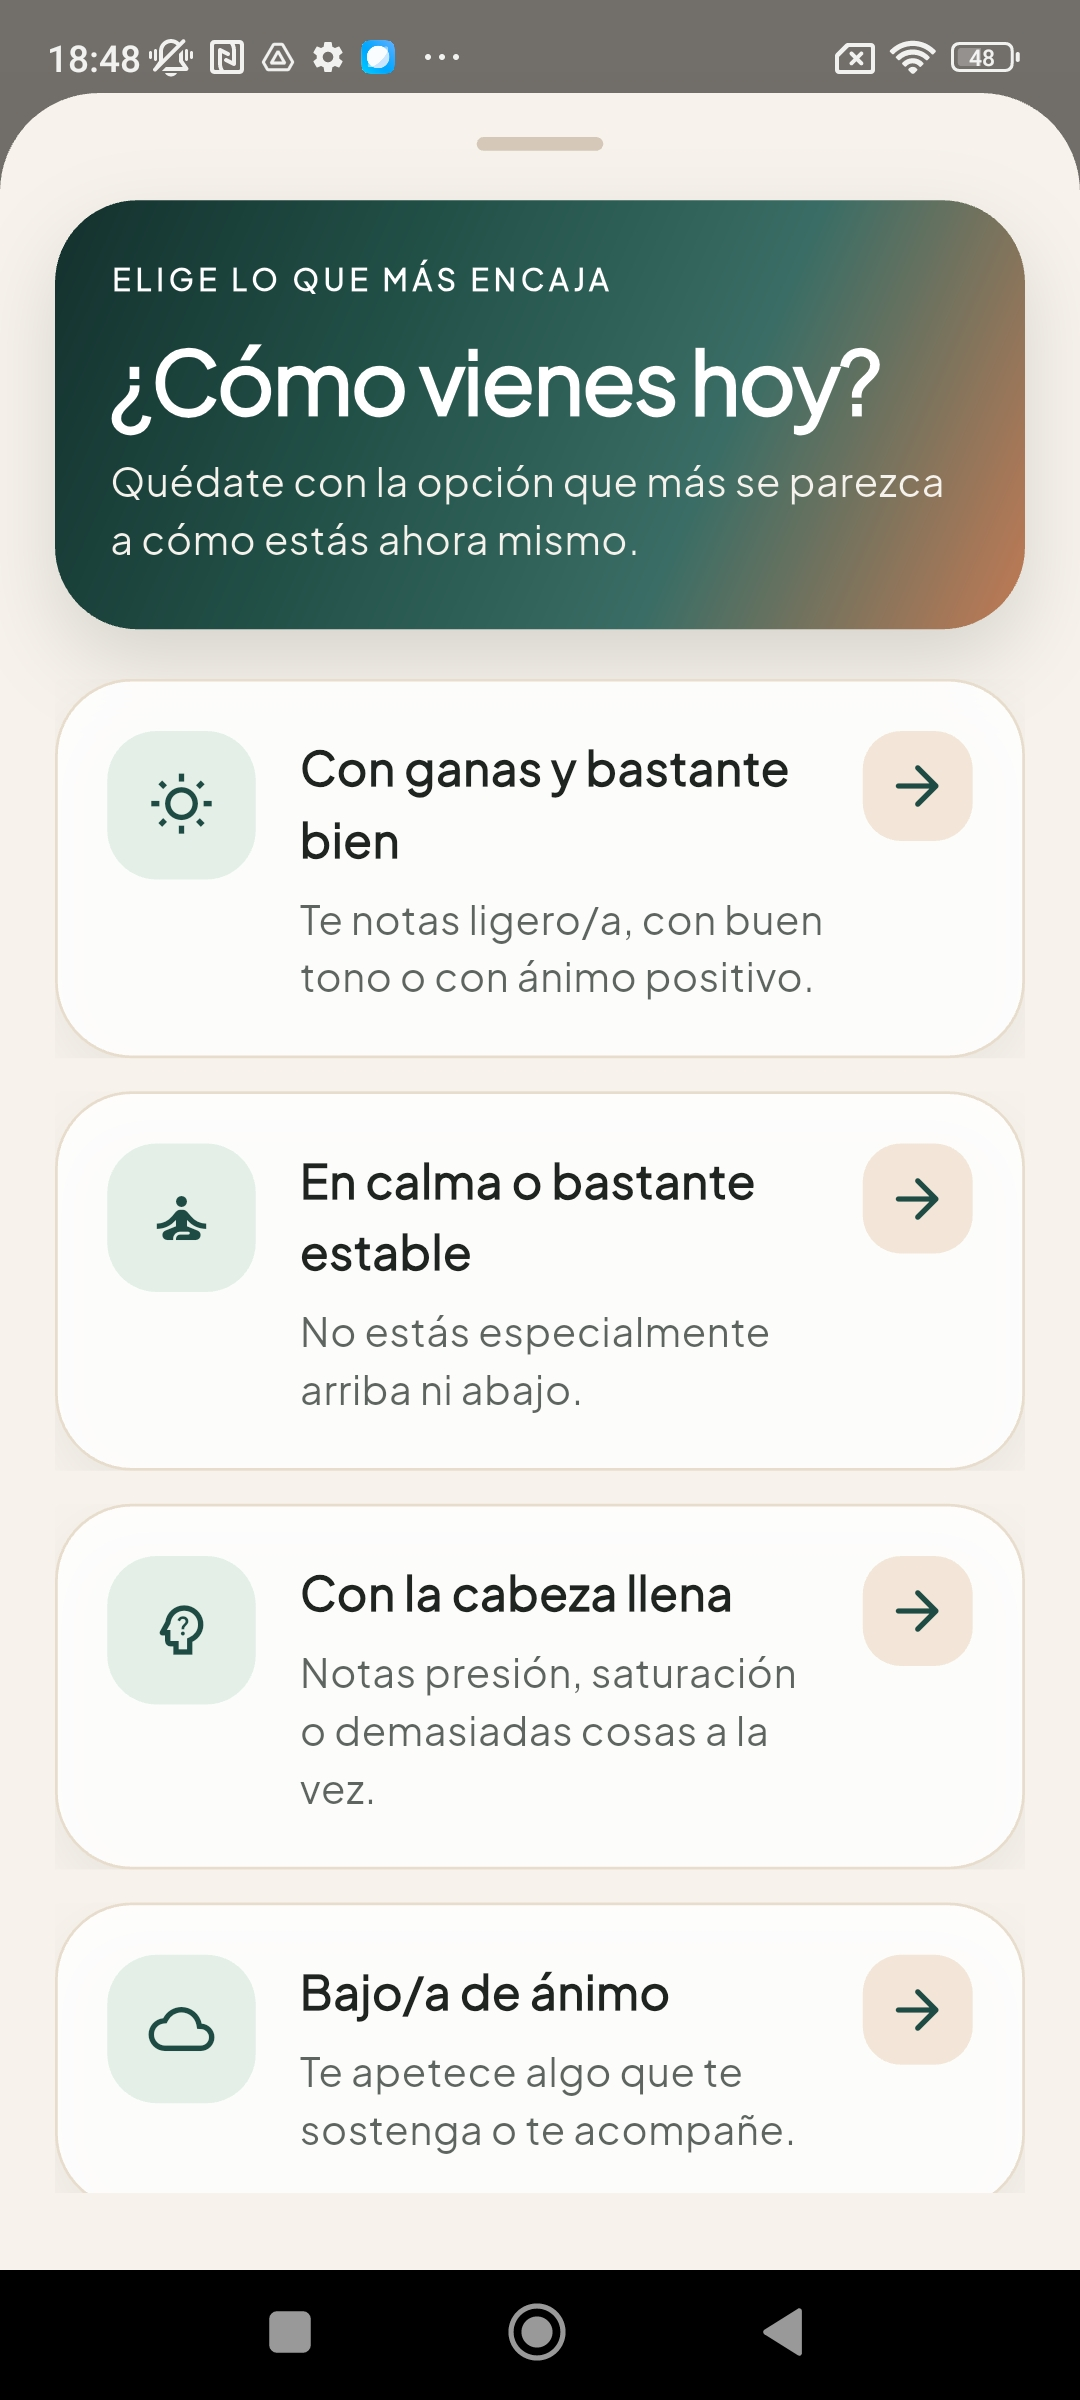
\includegraphics[width=\linewidth]{Imagenes/manual_app/Screenshot_2026-05-25-18-48-36-091_com.example.harmonyhub.jpg}
    \end{minipage}
    \caption{Pantalla principal y comienzo del check-in. A la izquierda se ve
    la portada con acceso directo a \textit{Empezar check-in}; a la derecha,
    una de las preguntas guiadas del flujo conversacional.}
    \label{fig:manual_home_checkin}
\end{figure}

La portada actúa como punto de entrada del producto. Desde ella se puede
empezar el check-in, consultar accesos a otros bloques y moverse por la
navegación inferior. Durante el check-in, Harmony Hub presenta preguntas breves
en lenguaje natural para recoger estado emocional, objetivo, energía, estrés y
preferencias sin exigir una interacción técnica.

\subsection*{Entorno acústico y generación de la recomendación}

\begin{figure}[htbp]
    \centering
    \begin{minipage}{0.47\textwidth}
        \centering
        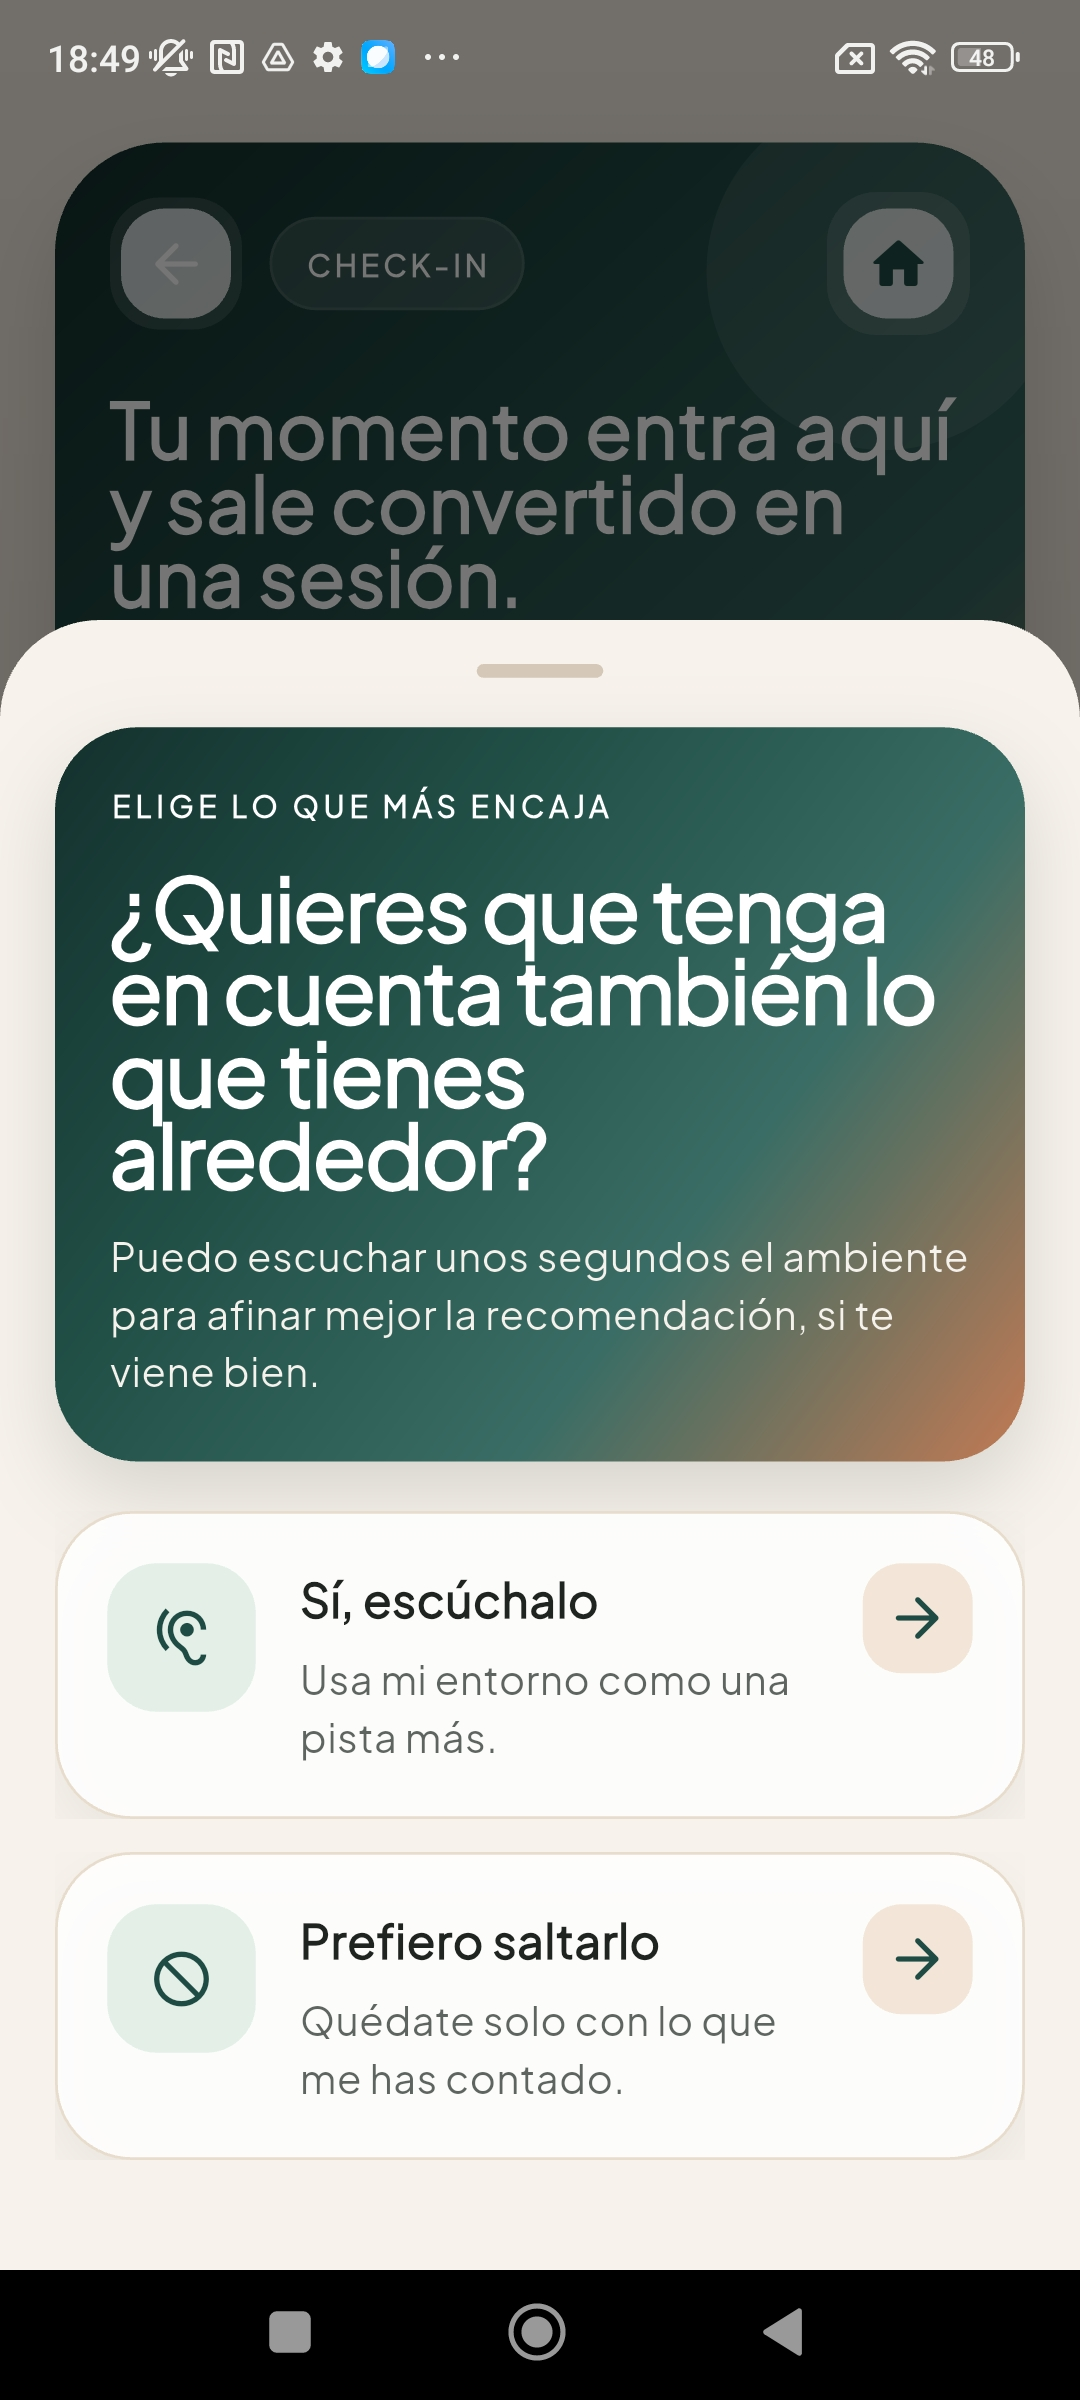
\includegraphics[width=\linewidth]{Imagenes/manual_app/Screenshot_2026-05-25-18-49-26-089_com.example.harmonyhub.jpg}
    \end{minipage}
    \hfill
    \begin{minipage}{0.47\textwidth}
        \centering
        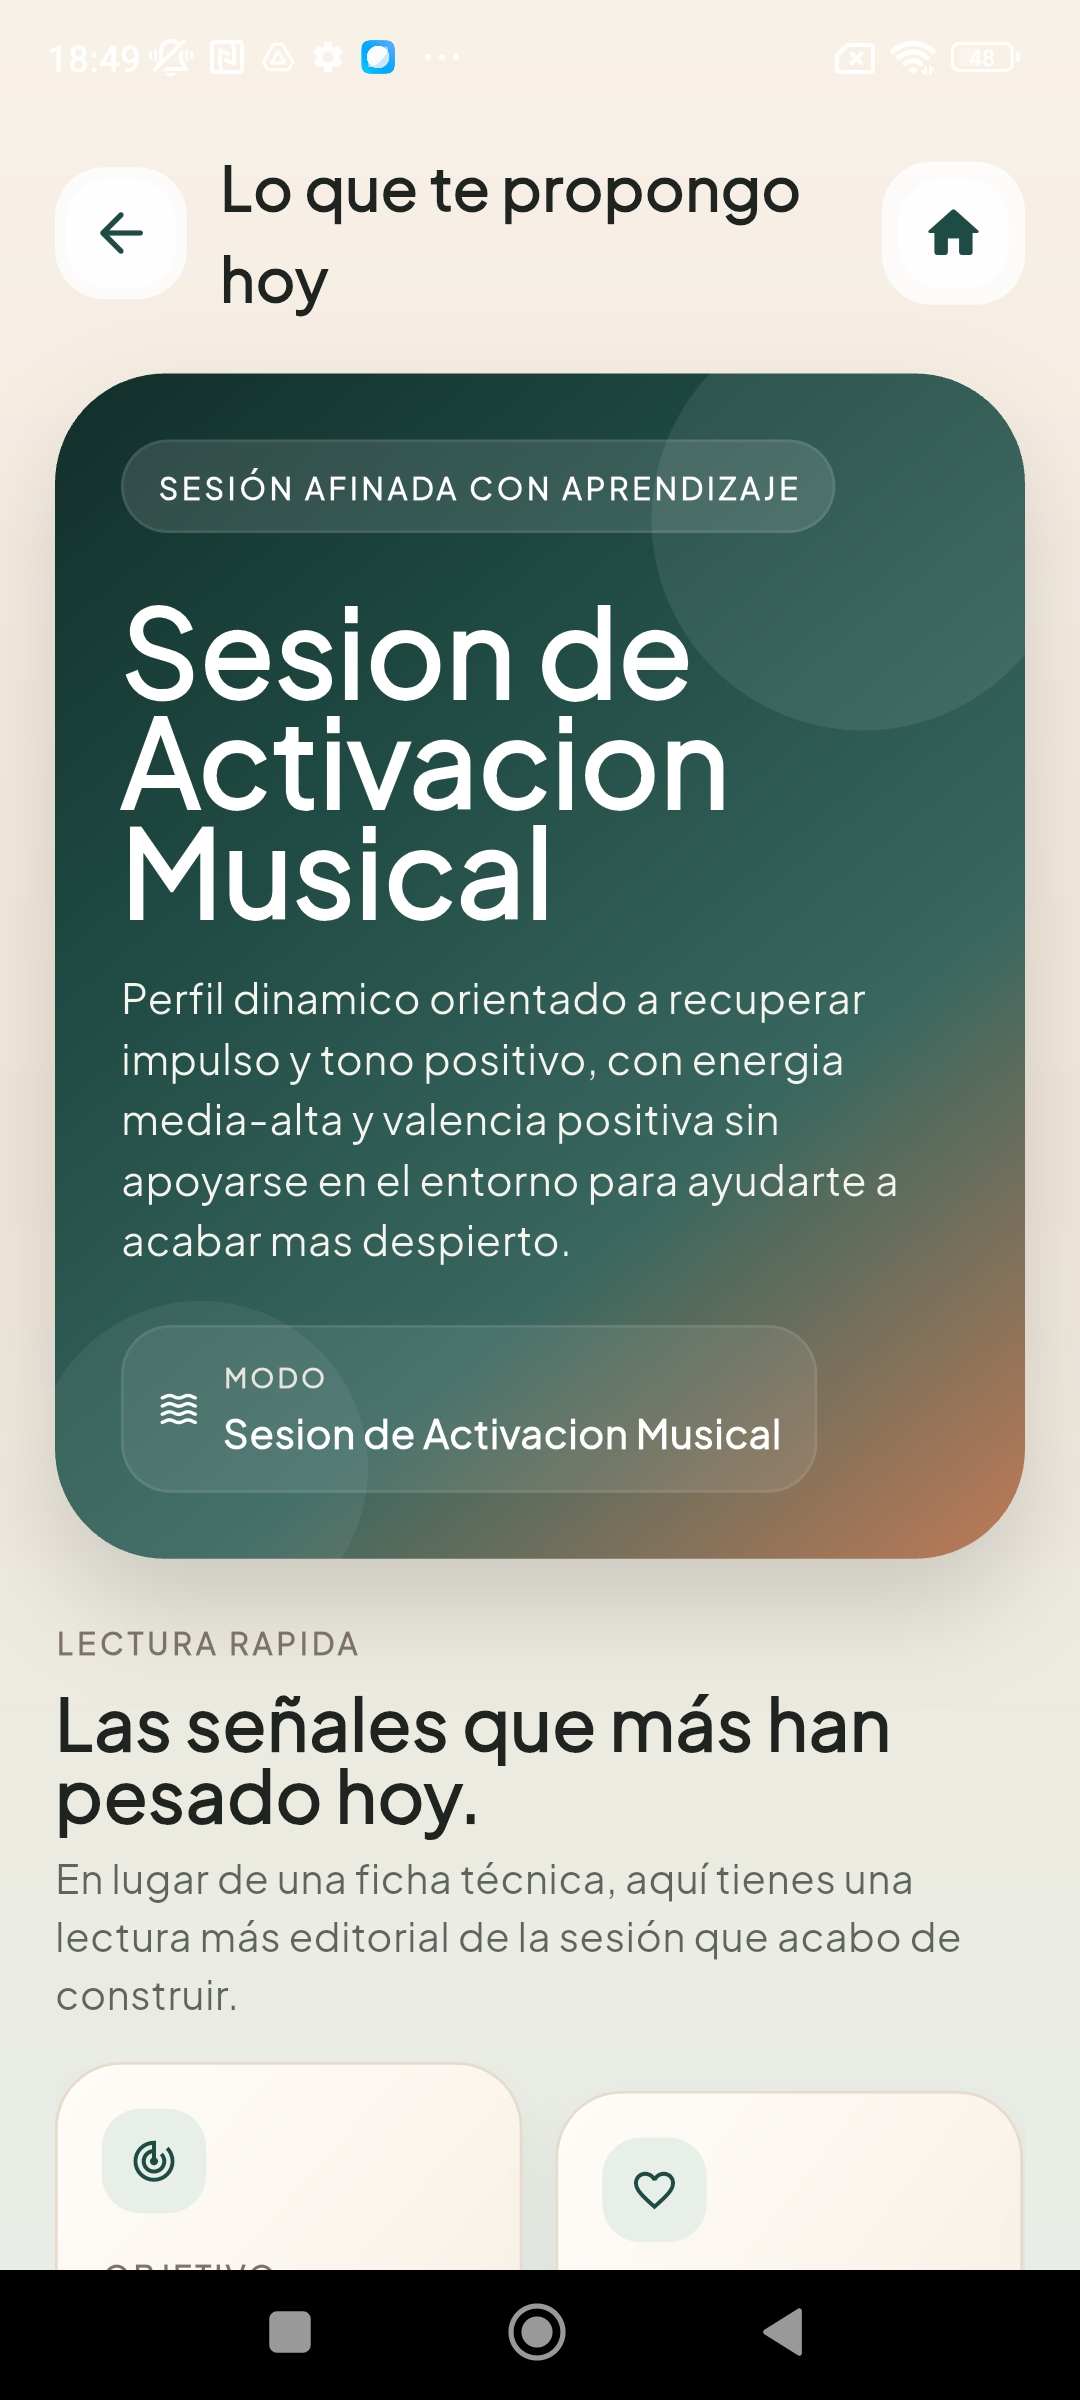
\includegraphics[width=\linewidth]{Imagenes/manual_app/Screenshot_2026-05-25-18-49-39-980_com.example.harmonyhub.jpg}
    \end{minipage}
    \caption{Activación opcional del análisis del entorno y presentación de la
    recomendación resultante.}
    \label{fig:manual_entorno_recomendacion}
\end{figure}

El análisis del entorno es opcional. Si la persona usuaria acepta, la app
escucha unos segundos el ambiente para utilizar esa señal como contexto
adicional. Después, se presenta una recomendación editorializada con el tipo de
sesión sugerido, una explicación funcional y un resumen del modo elegido.

\subsection*{Uso del aprendizaje acumulado y creación de la playlist}

\begin{figure}[htbp]
    \centering
    \begin{minipage}{0.47\textwidth}
        \centering
        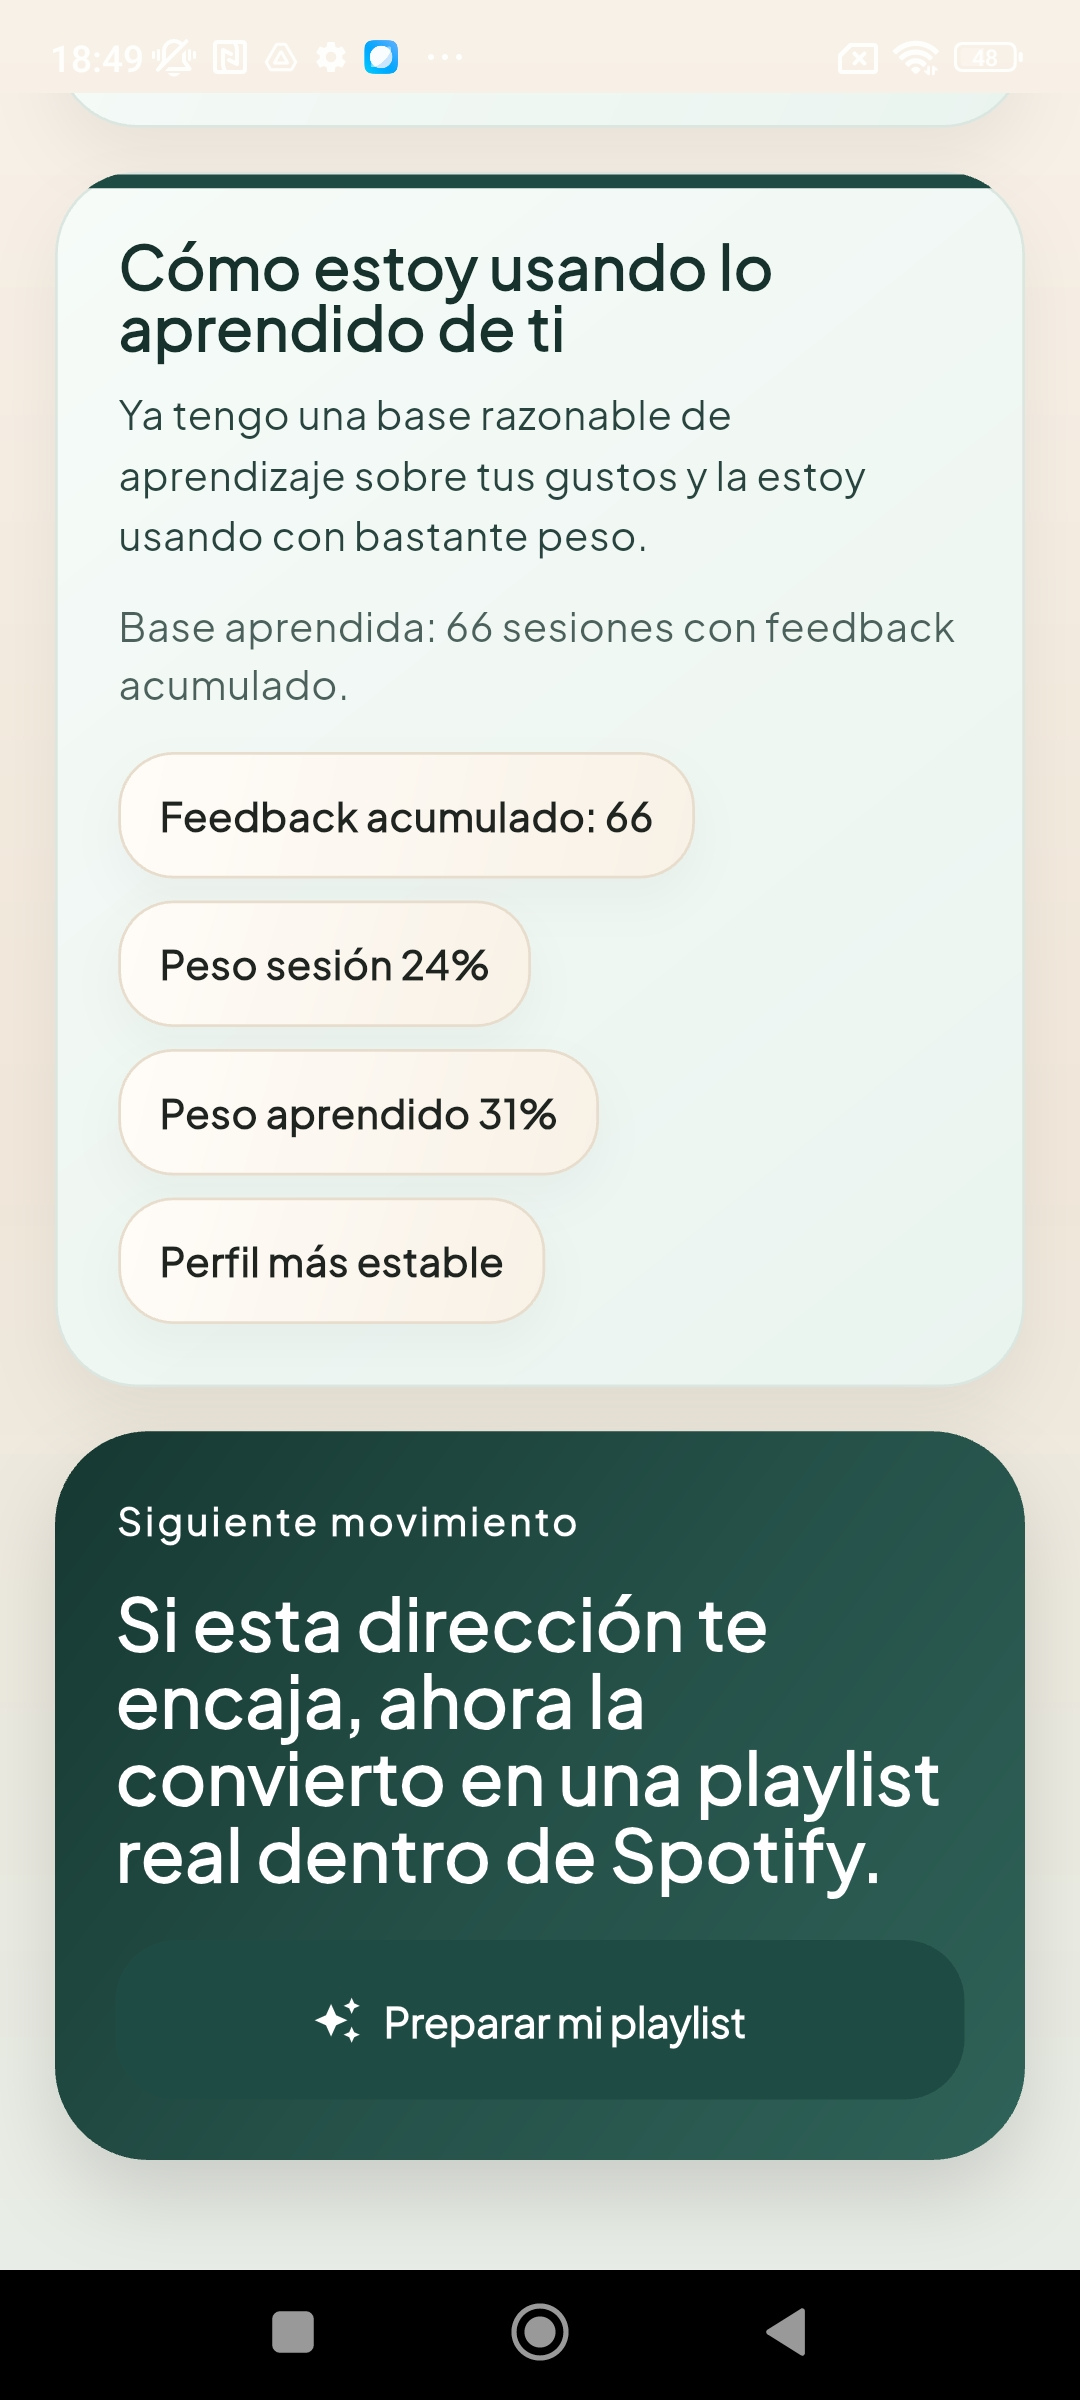
\includegraphics[width=\linewidth]{Imagenes/manual_app/Screenshot_2026-05-25-18-49-46-860_com.example.harmonyhub.jpg}
    \end{minipage}
    \hfill
    \begin{minipage}{0.47\textwidth}
        \centering
        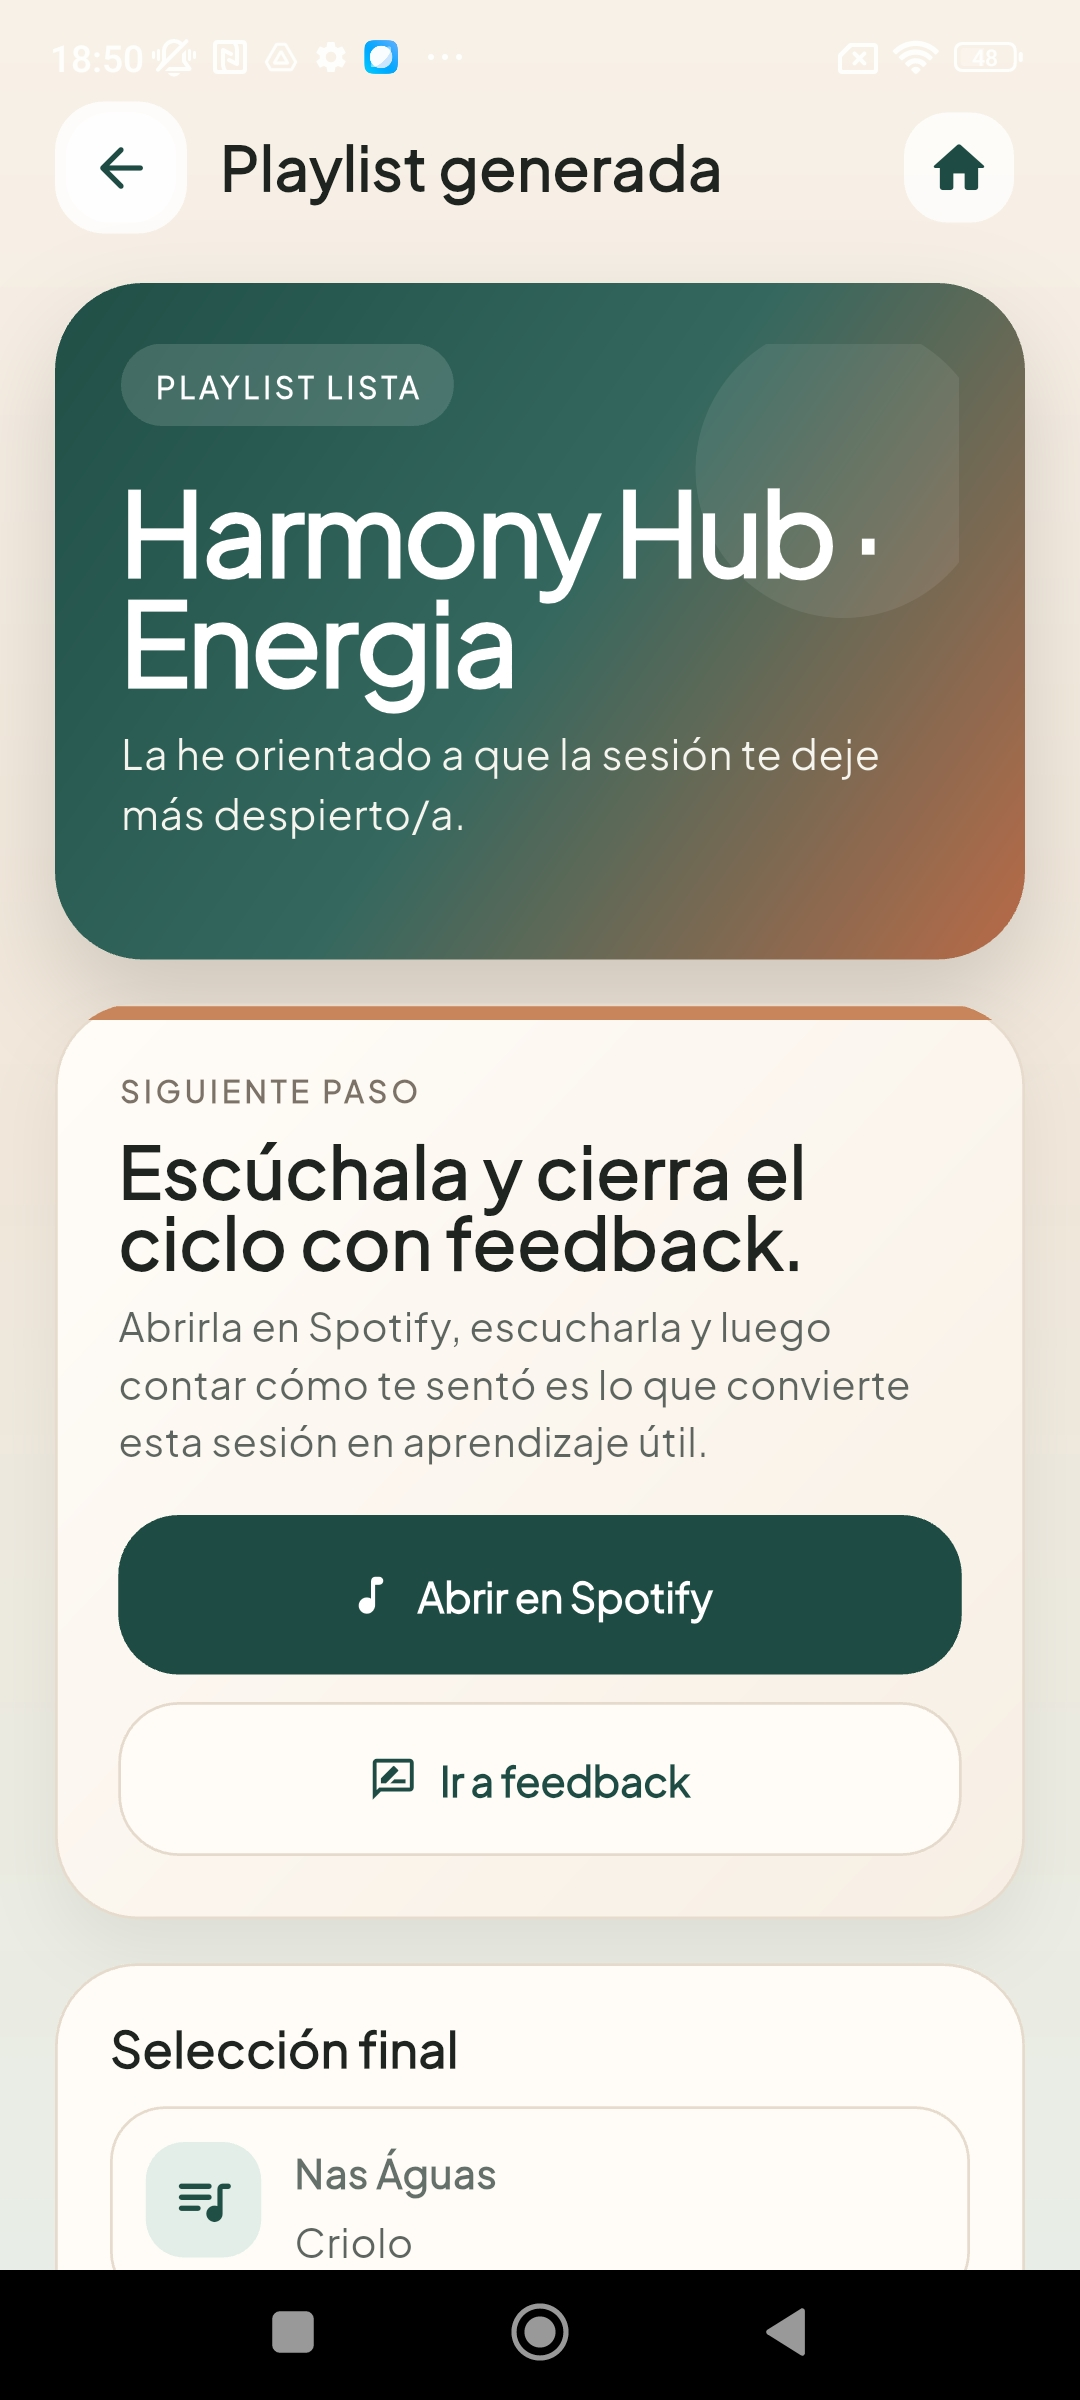
\includegraphics[width=\linewidth]{Imagenes/manual_app/Screenshot_2026-05-25-18-50-27-942_com.example.harmonyhub.jpg}
    \end{minipage}
    \caption{Explicación del peso del aprendizaje acumulado y pantalla de
    playlist ya generada dentro de la app.}
    \label{fig:manual_aprendizaje_playlist}
\end{figure}

Antes de crear la playlist, la recomendación puede mostrar cómo se está usando
el aprendizaje acumulado, incluyendo señales como el feedback disponible o el
peso relativo del perfil aprendido. Una vez generada la playlist, Harmony Hub
presenta el resultado final, permite abrirlo en Spotify y ofrece el acceso
directo al cierre con feedback.

\subsection*{Cierre de sesión y reproducción real en Spotify}

\begin{figure}[htbp]
    \centering
    \begin{minipage}{0.47\textwidth}
        \centering
        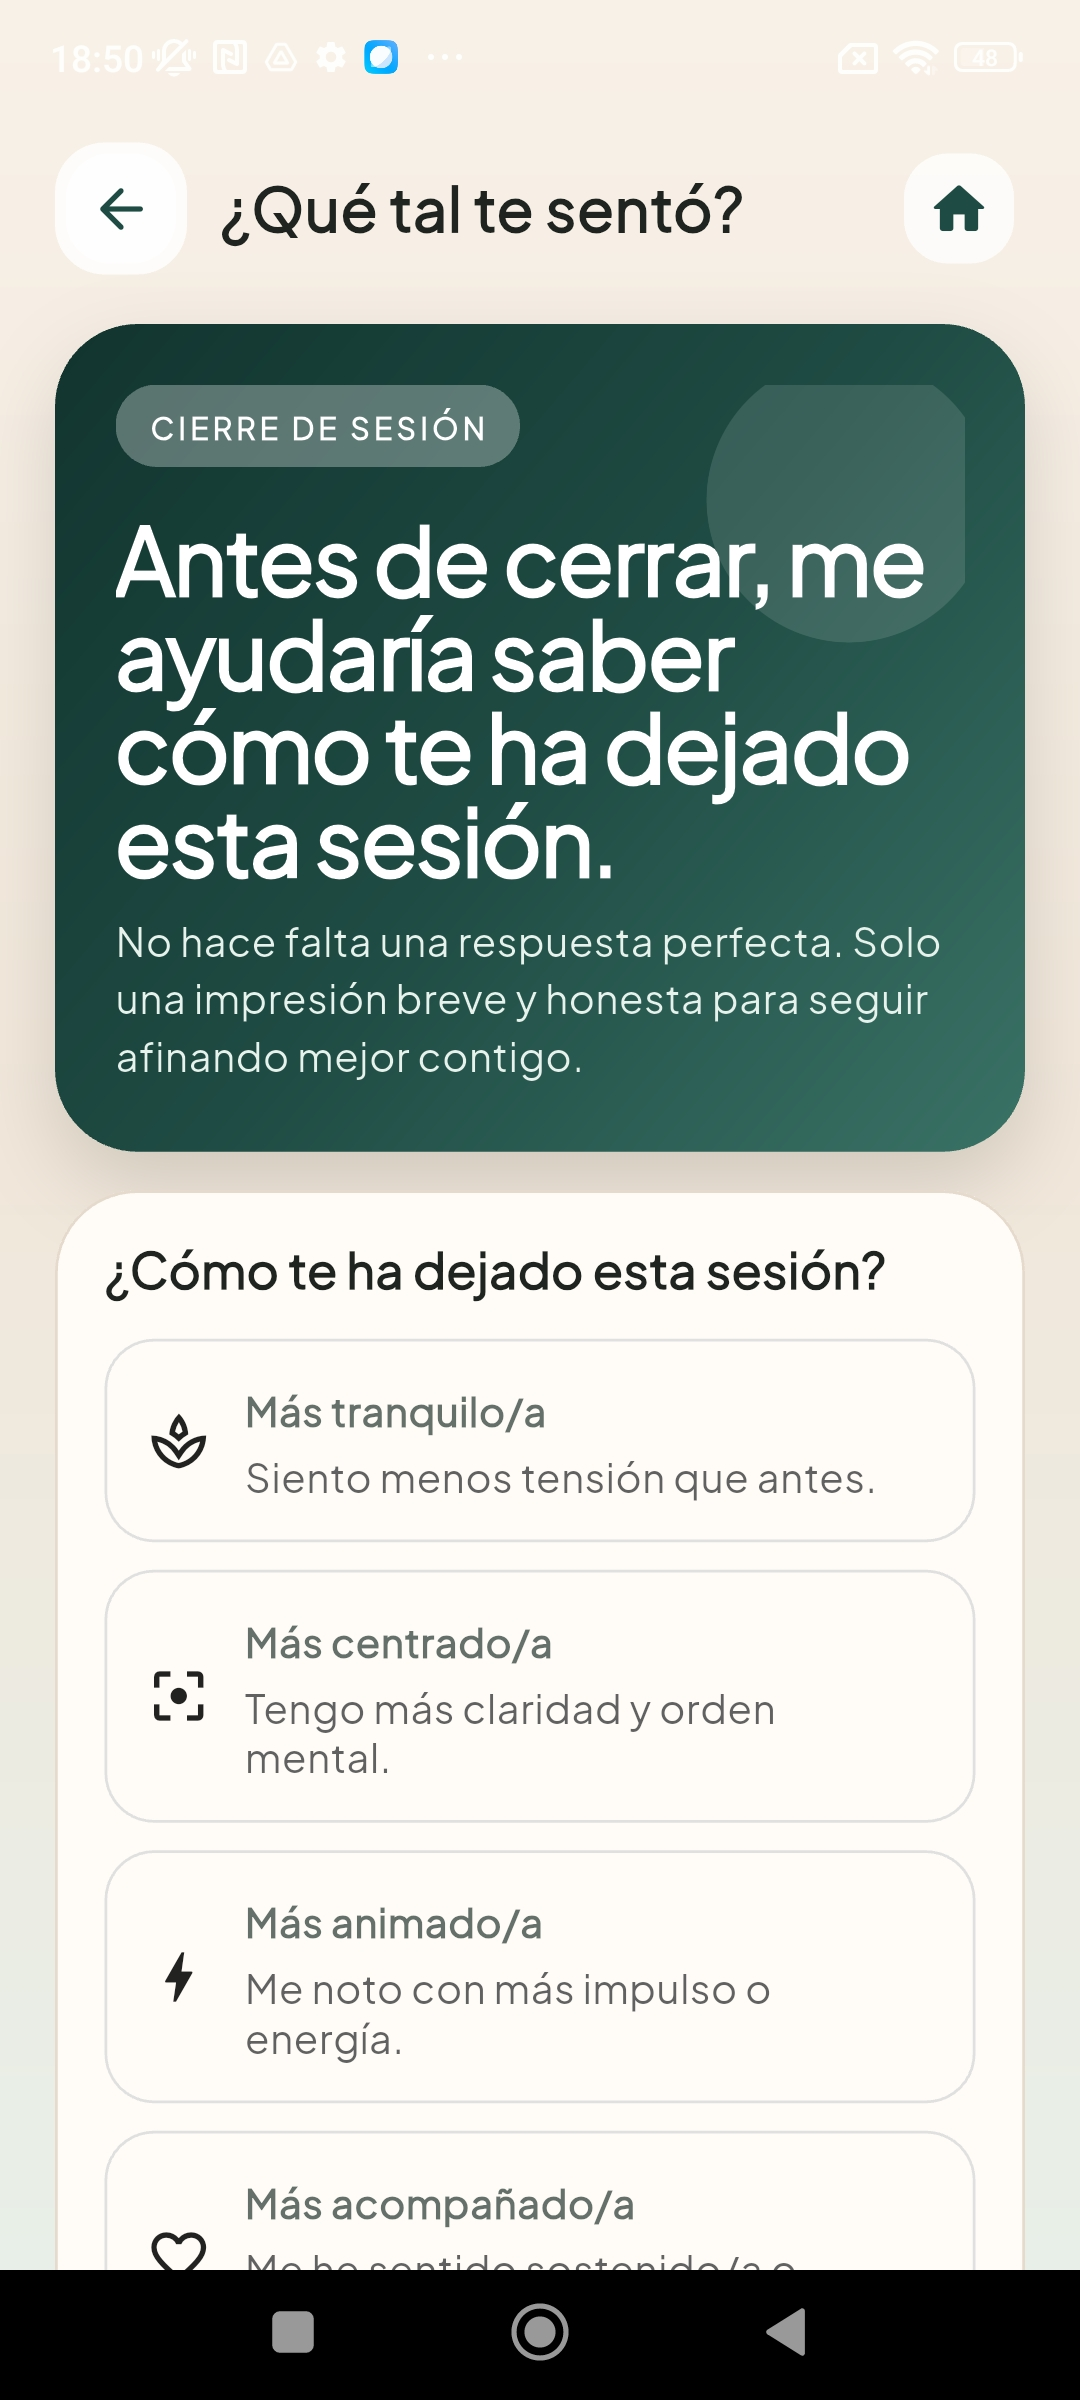
\includegraphics[width=\linewidth]{Imagenes/manual_app/Screenshot_2026-05-25-18-50-33-482_com.example.harmonyhub.jpg}
    \end{minipage}
    \hfill
    \begin{minipage}{0.47\textwidth}
        \centering
        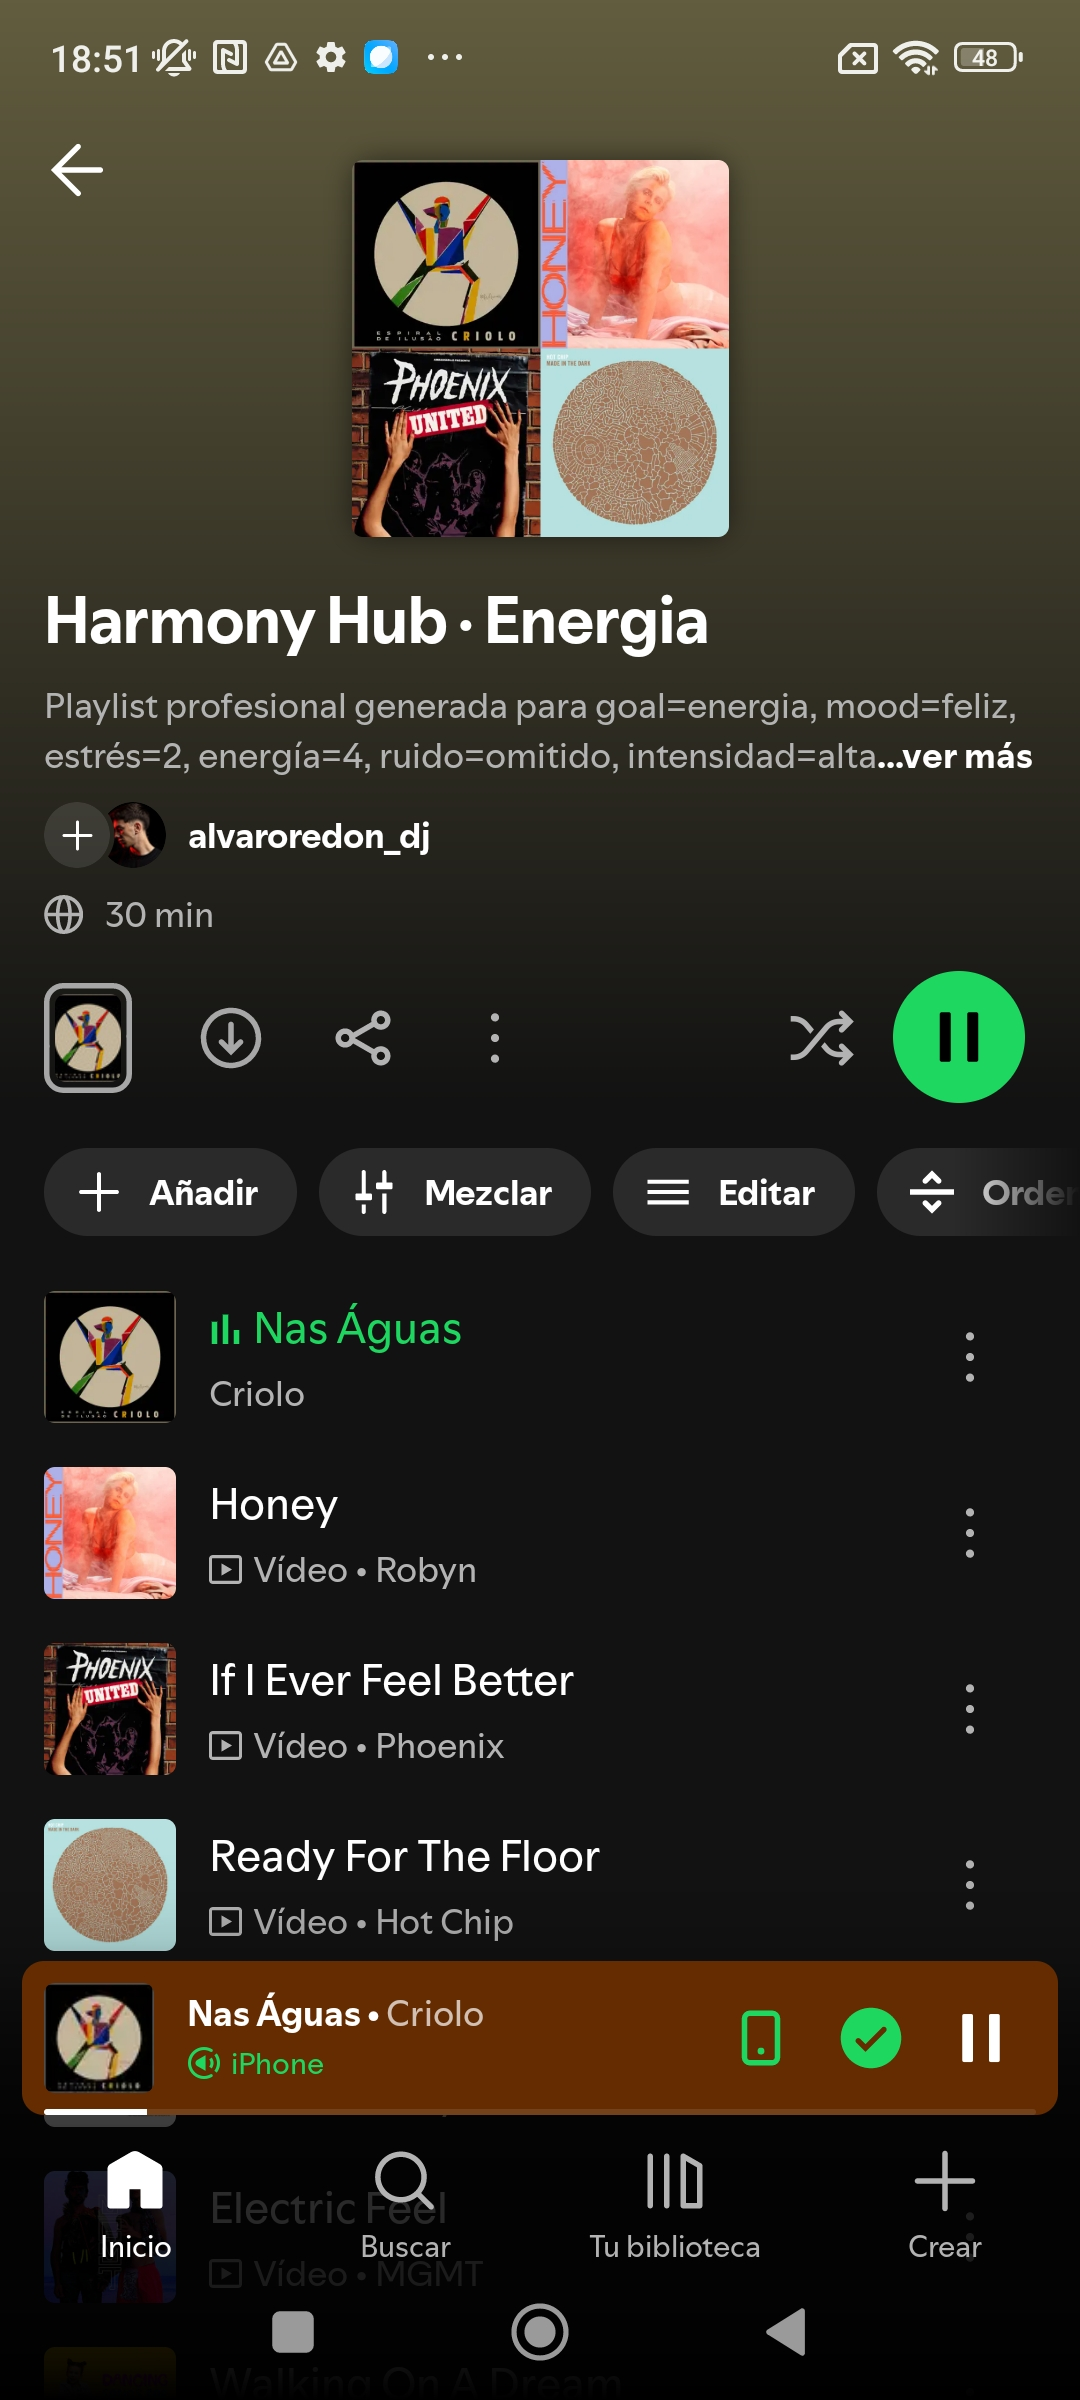
\includegraphics[width=\linewidth]{Imagenes/manual_app/Screenshot_2026-05-25-18-51-18-766_com.spotify.music.jpg}
    \end{minipage}
    \caption{Pantalla de feedback al cerrar la sesión y ejemplo de playlist
    abierta y reproducida ya dentro de Spotify.}
    \label{fig:manual_feedback_spotify}
\end{figure}

El ciclo de uso se cierra cuando la persona usuaria escucha la playlist y
responde cómo le ha dejado la sesión. Esta interacción es clave para el
aprendizaje posterior. La segunda imagen confirma además que la salida no se
queda en una sugerencia abstracta, sino que acaba convertida en una playlist
real dentro del ecosistema de Spotify.

\subsection*{Errores frecuentes y cómo interpretarlos}

Además del flujo correcto, resulta útil que la persona usuaria reconozca
algunos fallos previsibles y sepa qué significan. Las capturas siguientes no
representan errores arbitrarios, sino situaciones reales que pueden aparecer
durante el uso de la app y que conviene interpretar correctamente.

\begin{figure}[htbp]
    \centering
    \begin{minipage}{0.47\textwidth}
        \centering
        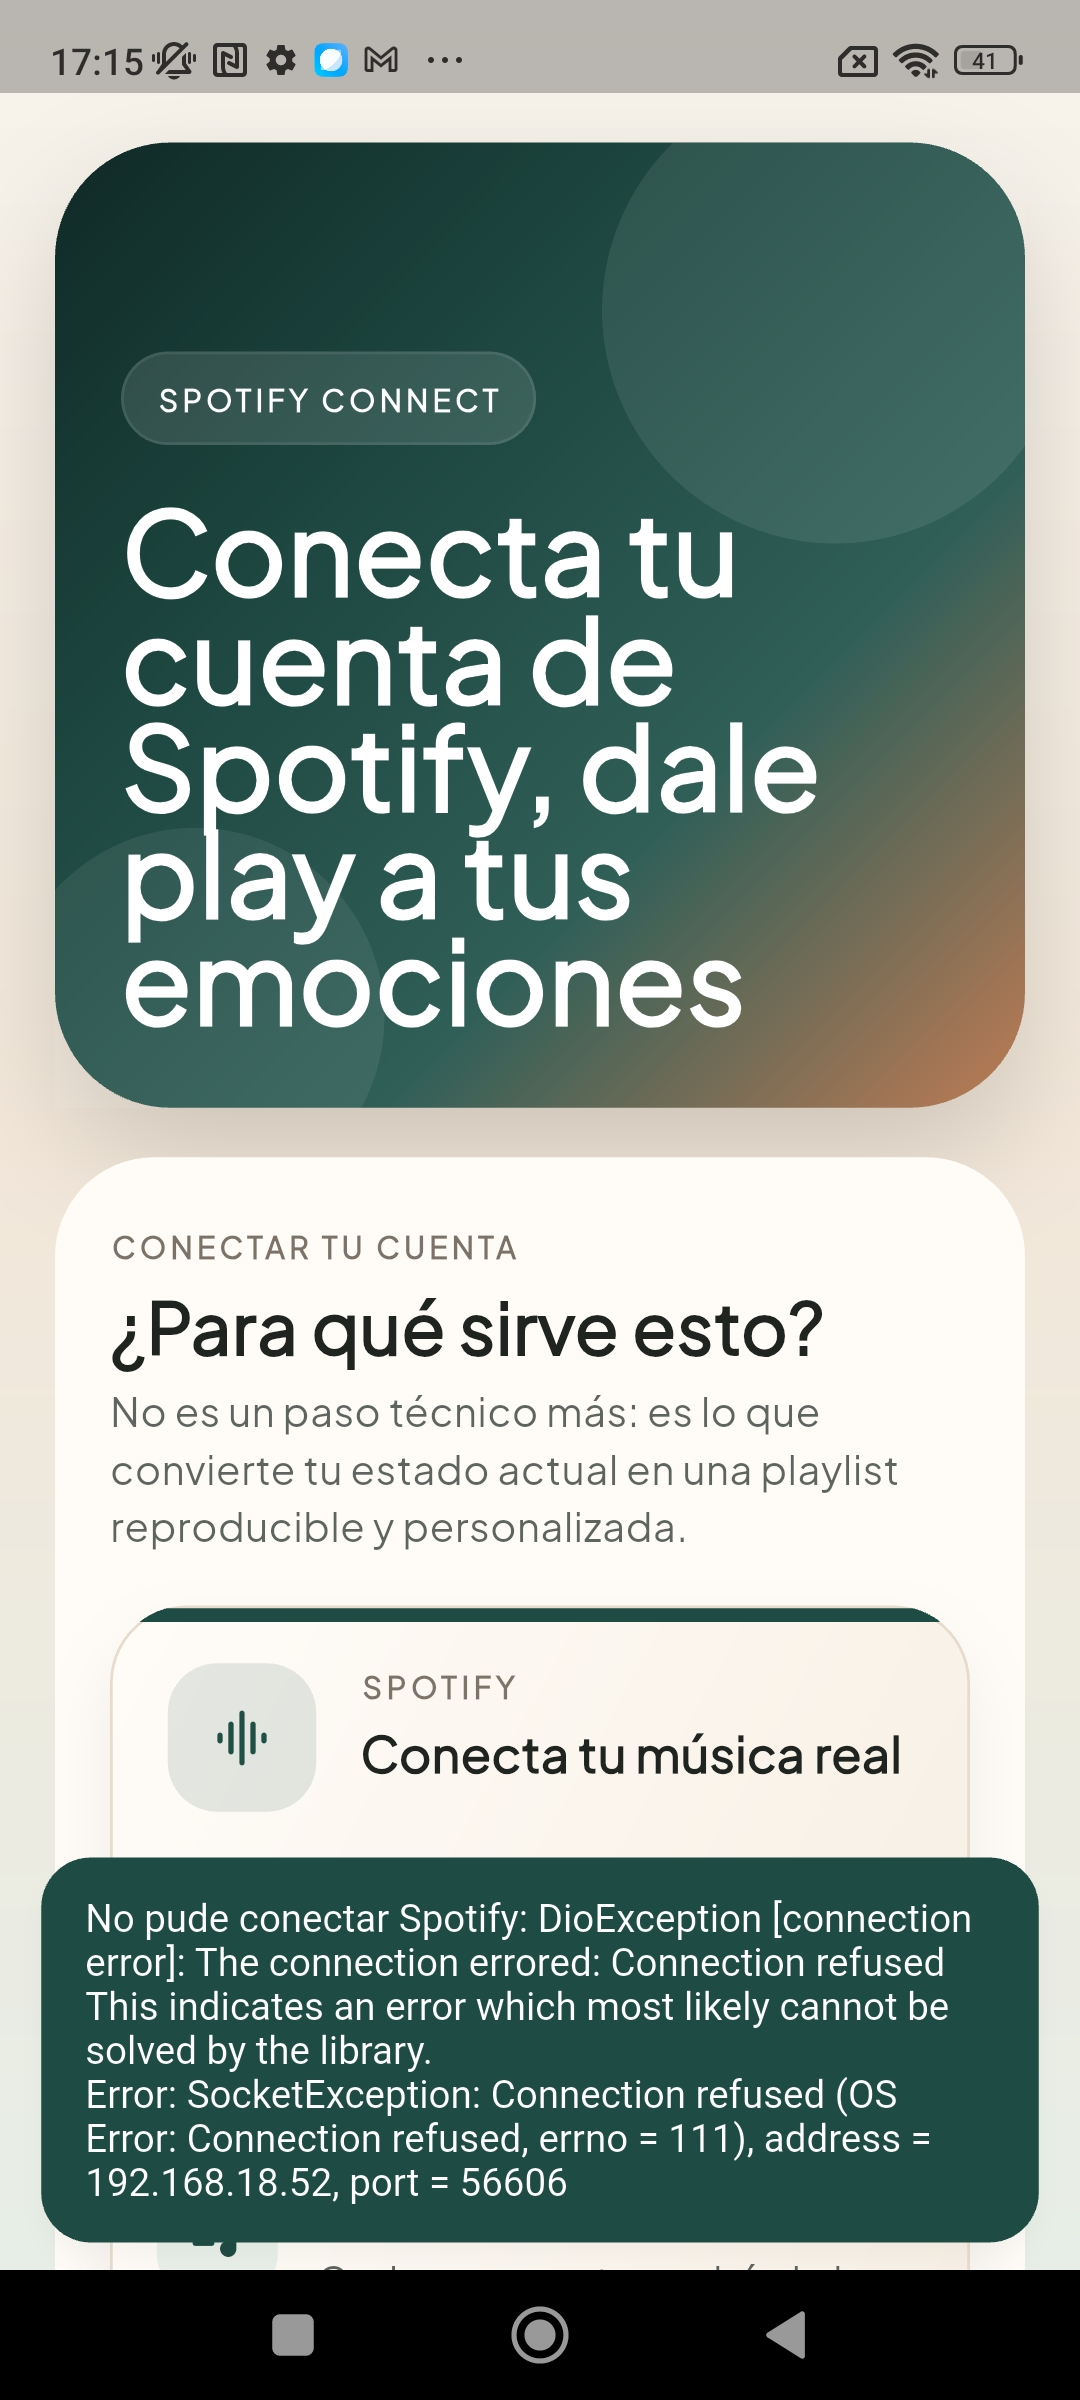
\includegraphics[width=\linewidth]{Imagenes/manual_errores/Screenshot_2026-05-26-17-15-11-055_com.example.harmonyhub.jpg}
    \end{minipage}
    \hfill
    \begin{minipage}{0.47\textwidth}
        \centering
        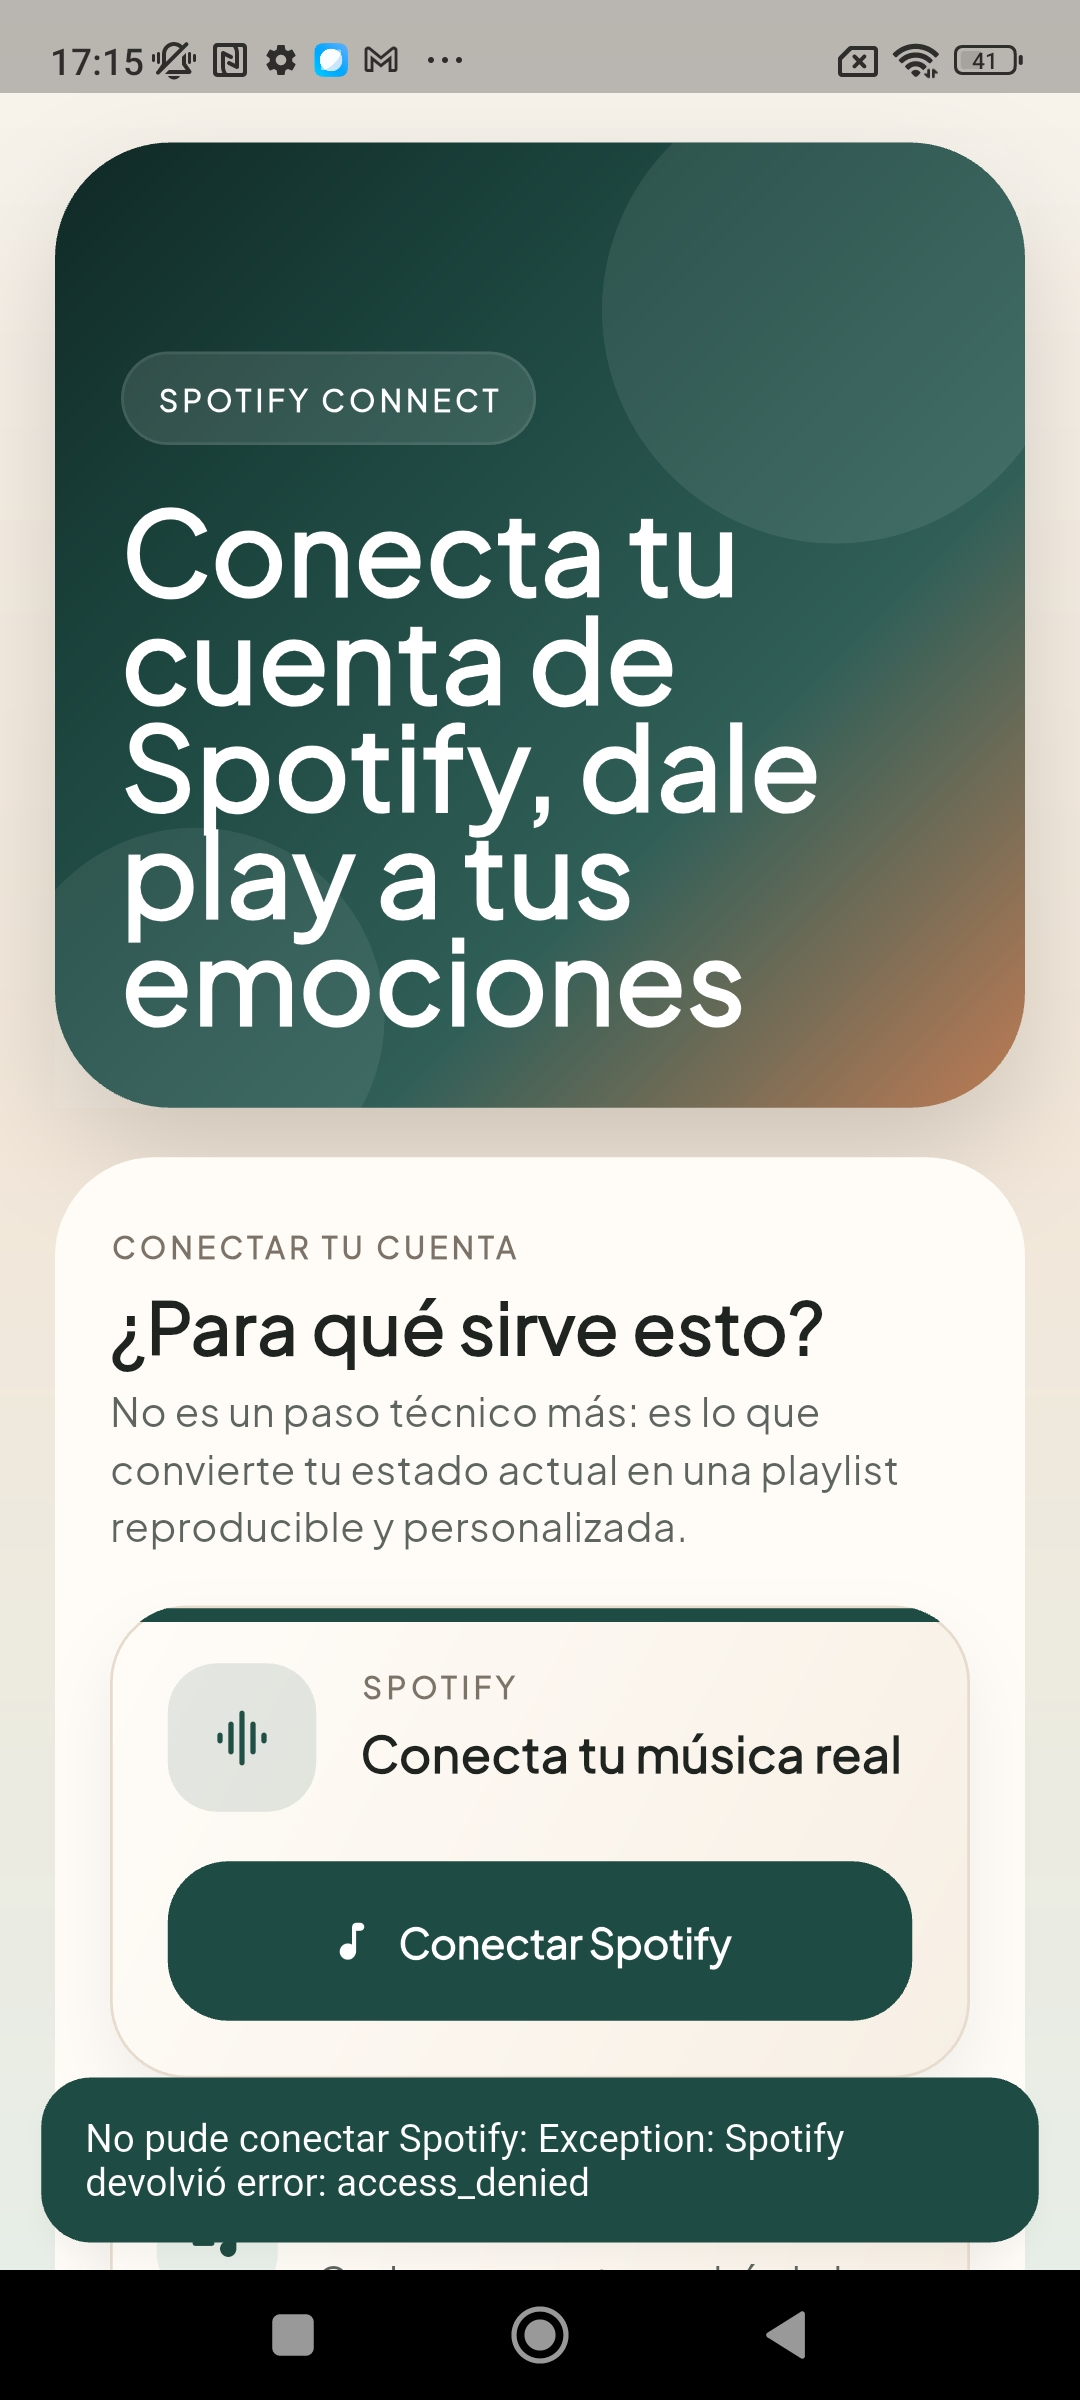
\includegraphics[width=\linewidth]{Imagenes/manual_errores/Screenshot_2026-05-26-17-15-35-245_com.example.harmonyhub.jpg}
    \end{minipage}
    \caption{Dos fallos posibles durante la conexión con Spotify: a la
    izquierda, error de comunicación con el backend local; a la derecha,
    cancelación o denegación del permiso por parte de Spotify.}
    \label{fig:manual_errores_spotify}
\end{figure}

La figura~\ref{fig:manual_errores_spotify} reúne dos casos distintos. En la
primera imagen, Harmony Hub no puede alcanzar el backend y por eso falla el
inicio del flujo OAuth. En una demostración real, esta situación suele
corregirse comprobando que el backend está activo y accesible desde la misma
red que el móvil. En la segunda imagen, el backend sí responde, pero Spotify
devuelve \texttt{access\_denied}; esto significa que la autorización fue
cancelada o rechazada y basta con volver a iniciar la conexión y aceptar el
permiso.

\begin{figure}[htbp]
    \centering
    \begin{minipage}{0.47\textwidth}
        \centering
        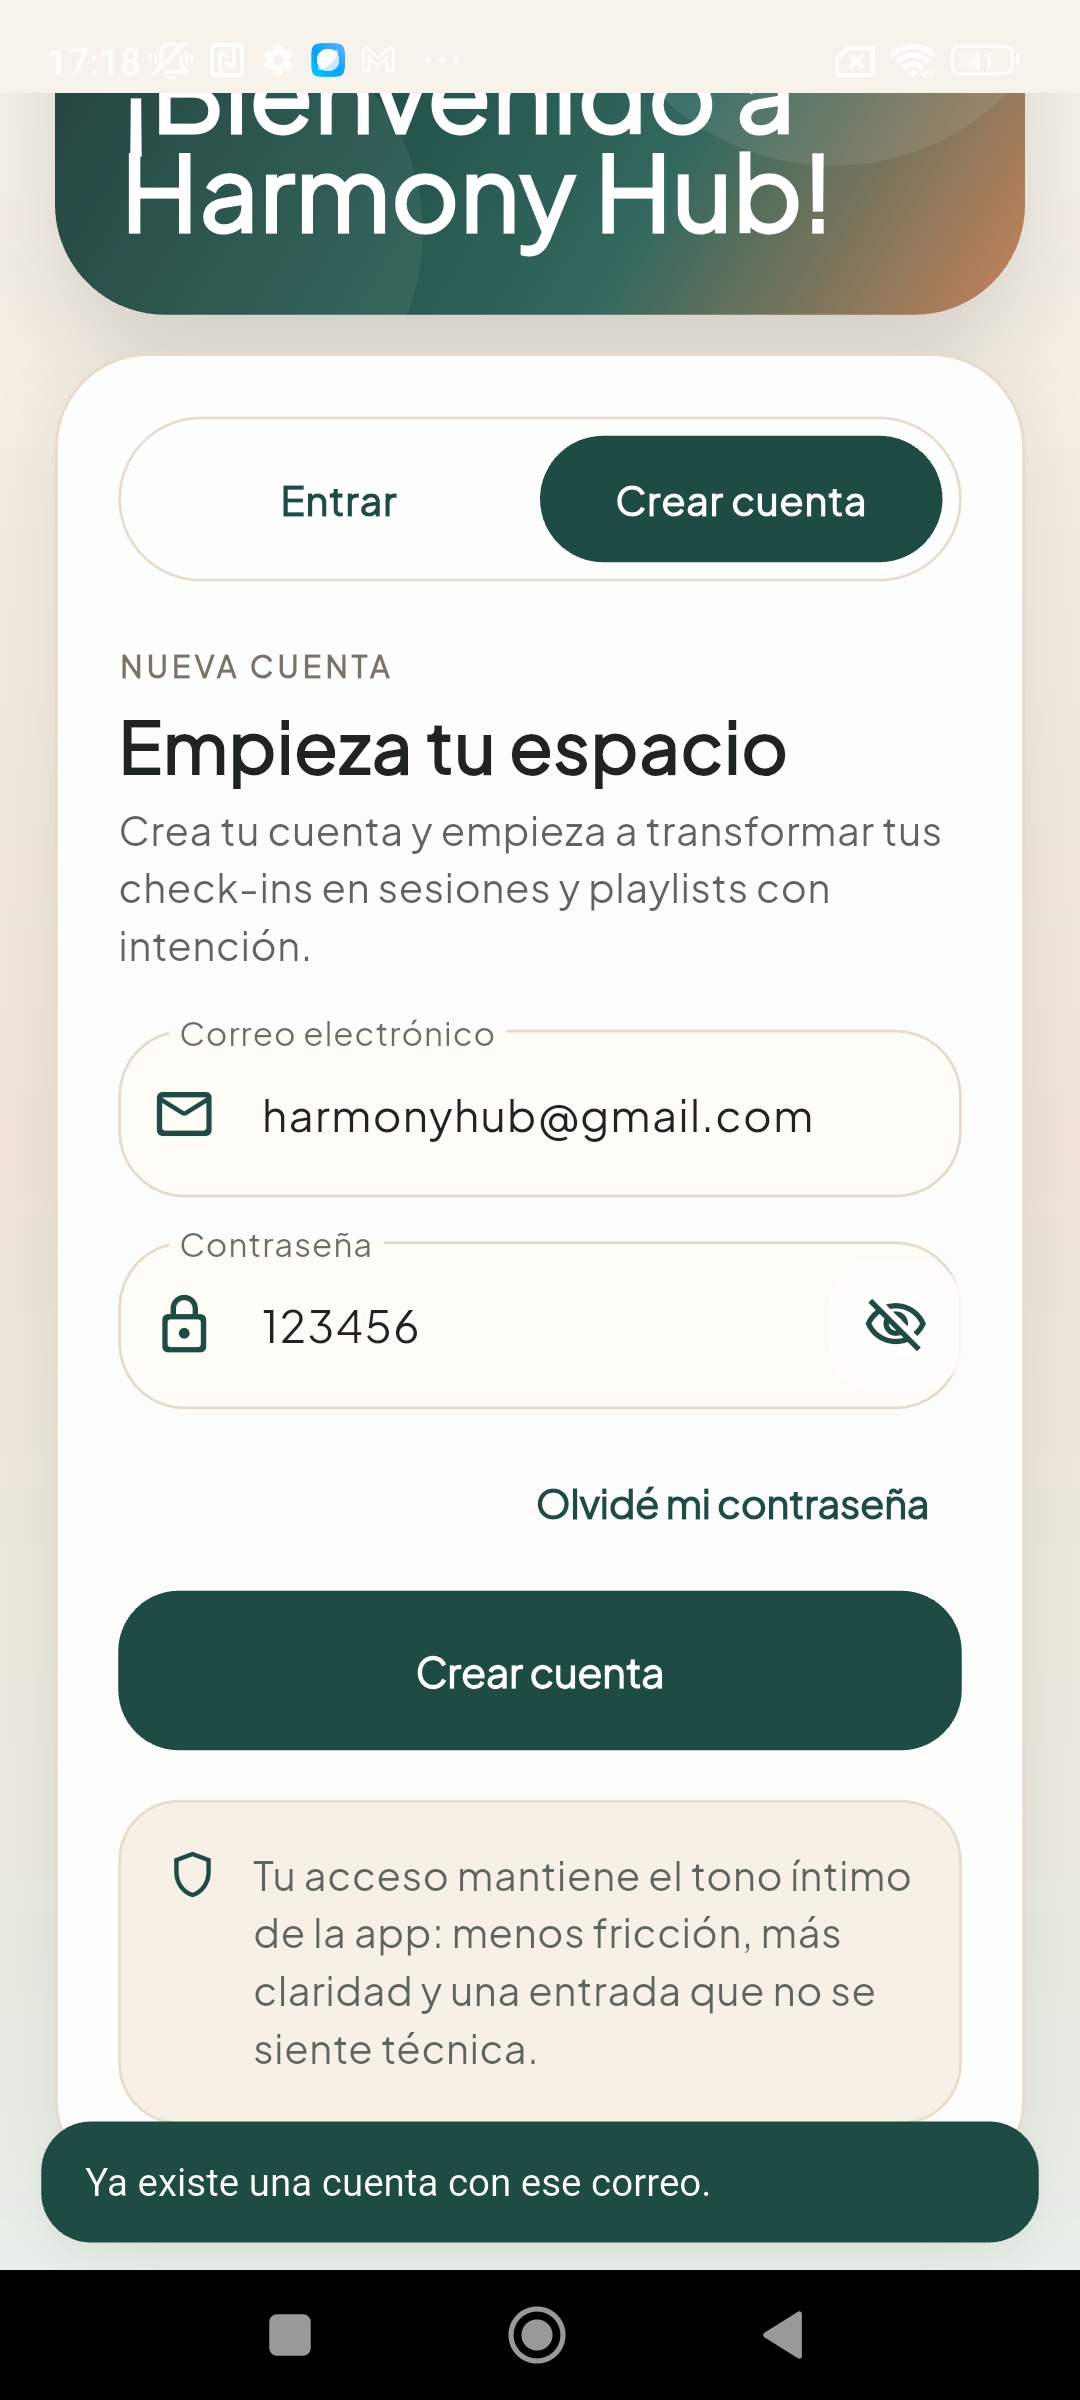
\includegraphics[width=\linewidth]{Imagenes/manual_errores/Screenshot_2026-05-26-17-18-25-628_com.example.harmonyhub.jpg}
    \end{minipage}
    \hfill
    \begin{minipage}{0.47\textwidth}
        \centering
        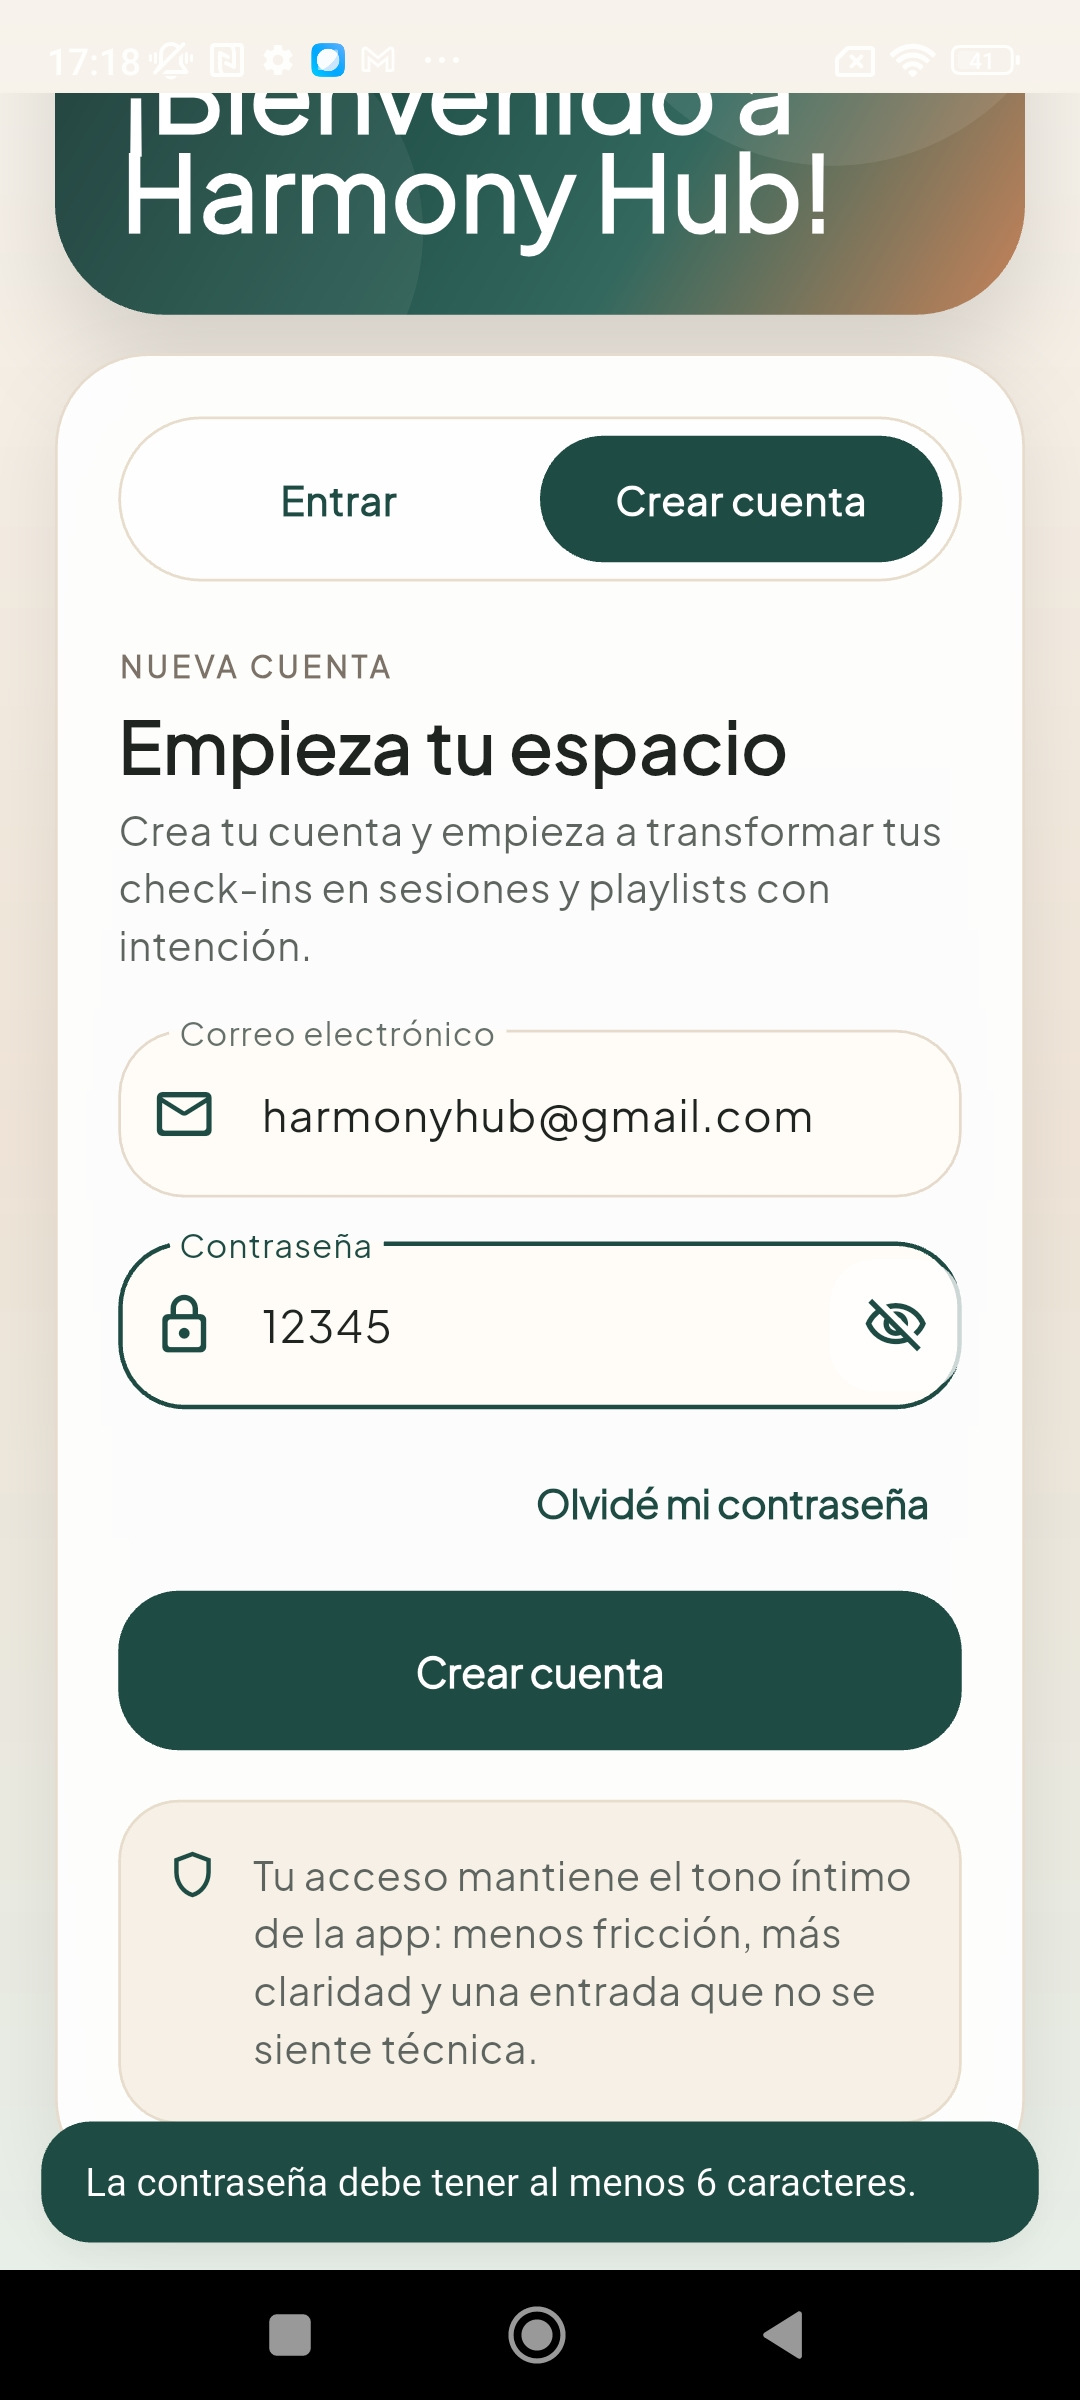
\includegraphics[width=\linewidth]{Imagenes/manual_errores/Screenshot_2026-05-26-17-18-40-964_com.example.harmonyhub.jpg}
    \end{minipage}
    \caption{Validaciones inmediatas del bloque de autenticación: cuenta ya
    existente y contraseña demasiado corta.}
    \label{fig:manual_errores_auth}
\end{figure}

La figura~\ref{fig:manual_errores_auth} muestra dos validaciones sencillas pero
útiles de cara a la experiencia de usuario. La primera evita crear una cuenta
duplicada con un correo que ya existe. La segunda recuerda que la contraseña
debe cumplir una longitud mínima antes de continuar. Ambas validaciones ayudan
a prevenir errores de entrada sin esperar a fases posteriores del flujo.

\begin{figure}[htbp]
    \centering
    \begin{minipage}{0.52\textwidth}
        \centering
        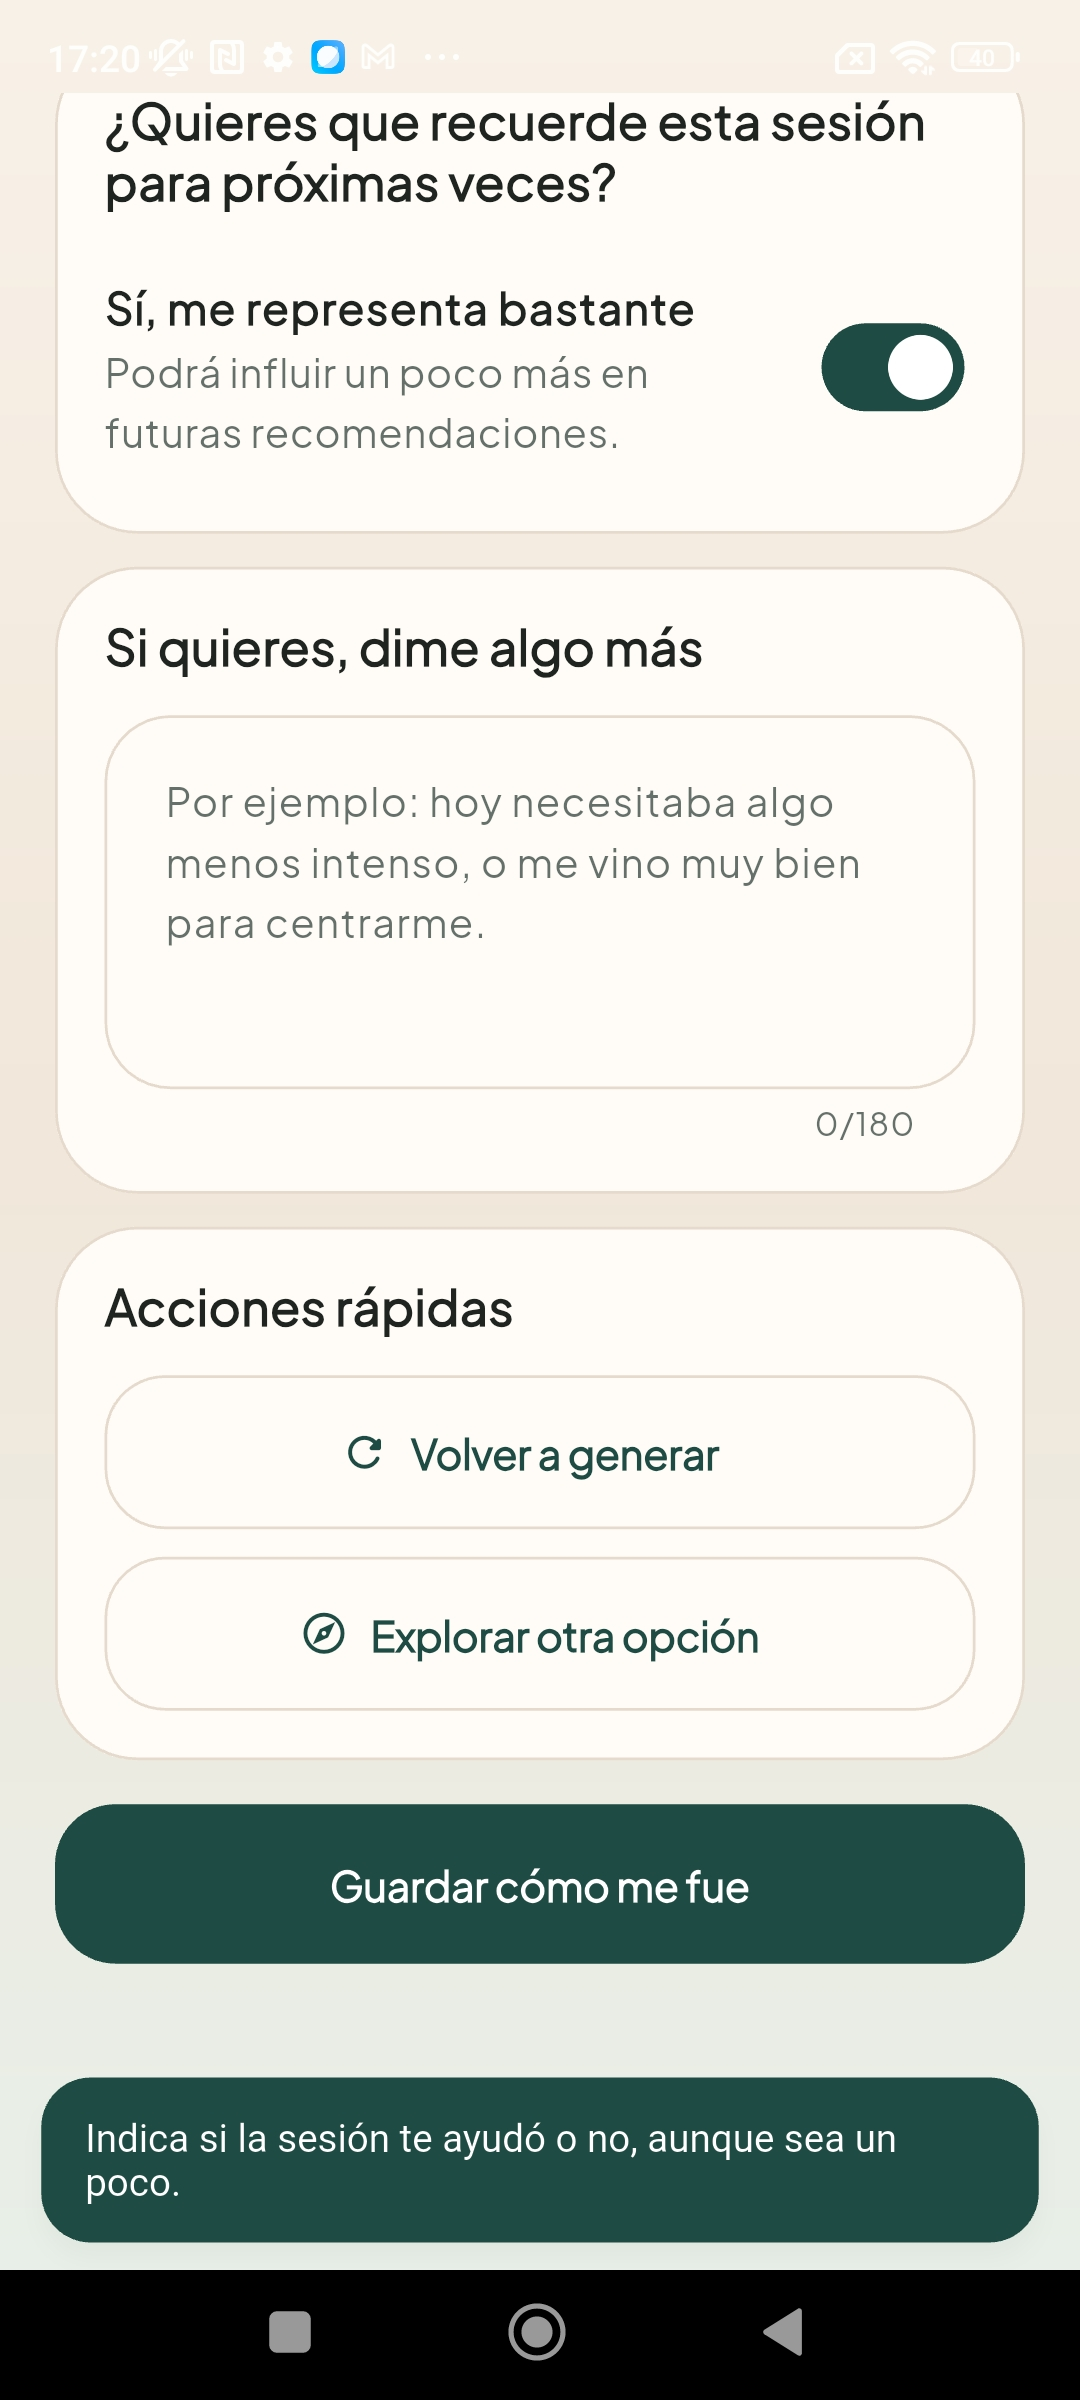
\includegraphics[width=\linewidth]{Imagenes/manual_errores/Screenshot_2026-05-26-17-20-39-922_com.example.harmonyhub.jpg}
    \end{minipage}
    \caption{Validación en la pantalla de feedback cuando se intenta guardar la
    sesión sin indicar todavía si la recomendación ayudó o no.}
    \label{fig:manual_error_feedback}
\end{figure}

Por último, la figura~\ref{fig:manual_error_feedback} refleja un caso ligado al
aprendizaje posterior del sistema. Antes de guardar el cierre de sesión,
Harmony Hub exige que la persona usuaria indique si la experiencia le ayudó al
menos un poco. Esta comprobación tiene una doble utilidad: evita registros
incompletos y garantiza que el backend solo reciba feedback interpretable para
seguir ajustando el perfil aprendido y el componente supervisado.

\section{Funcionalidades principales}
\label{sec:manual_usuario_funcionalidades}

\subsection*{Check-in contextual}

Permite describir el momento actual del usuario mediante una interacción breve.
Es la puerta de entrada del sistema y condiciona la recomendación posterior.

\subsection*{Recomendación de sesión}

La app devuelve un modo sugerido y una explicación funcional del perfil
musical esperado. Esta recomendación puede apoyarse en reglas contextuales y,
cuando existe evidencia suficiente, en aprendizaje acumulado.

\subsection*{Generación de playlist en Spotify}

Si la cuenta está conectada correctamente, la recomendación puede materializarse
como playlist real dentro de Spotify. La aplicación crea la lista y enlaza su
identificador con la sesión correspondiente.

\subsection*{Historial}

El usuario puede revisar sesiones anteriores, playlists generadas y parte de la
trazabilidad funcional acumulada.

\begin{figure}[htbp]
    \centering
    \begin{minipage}{0.47\textwidth}
        \centering
        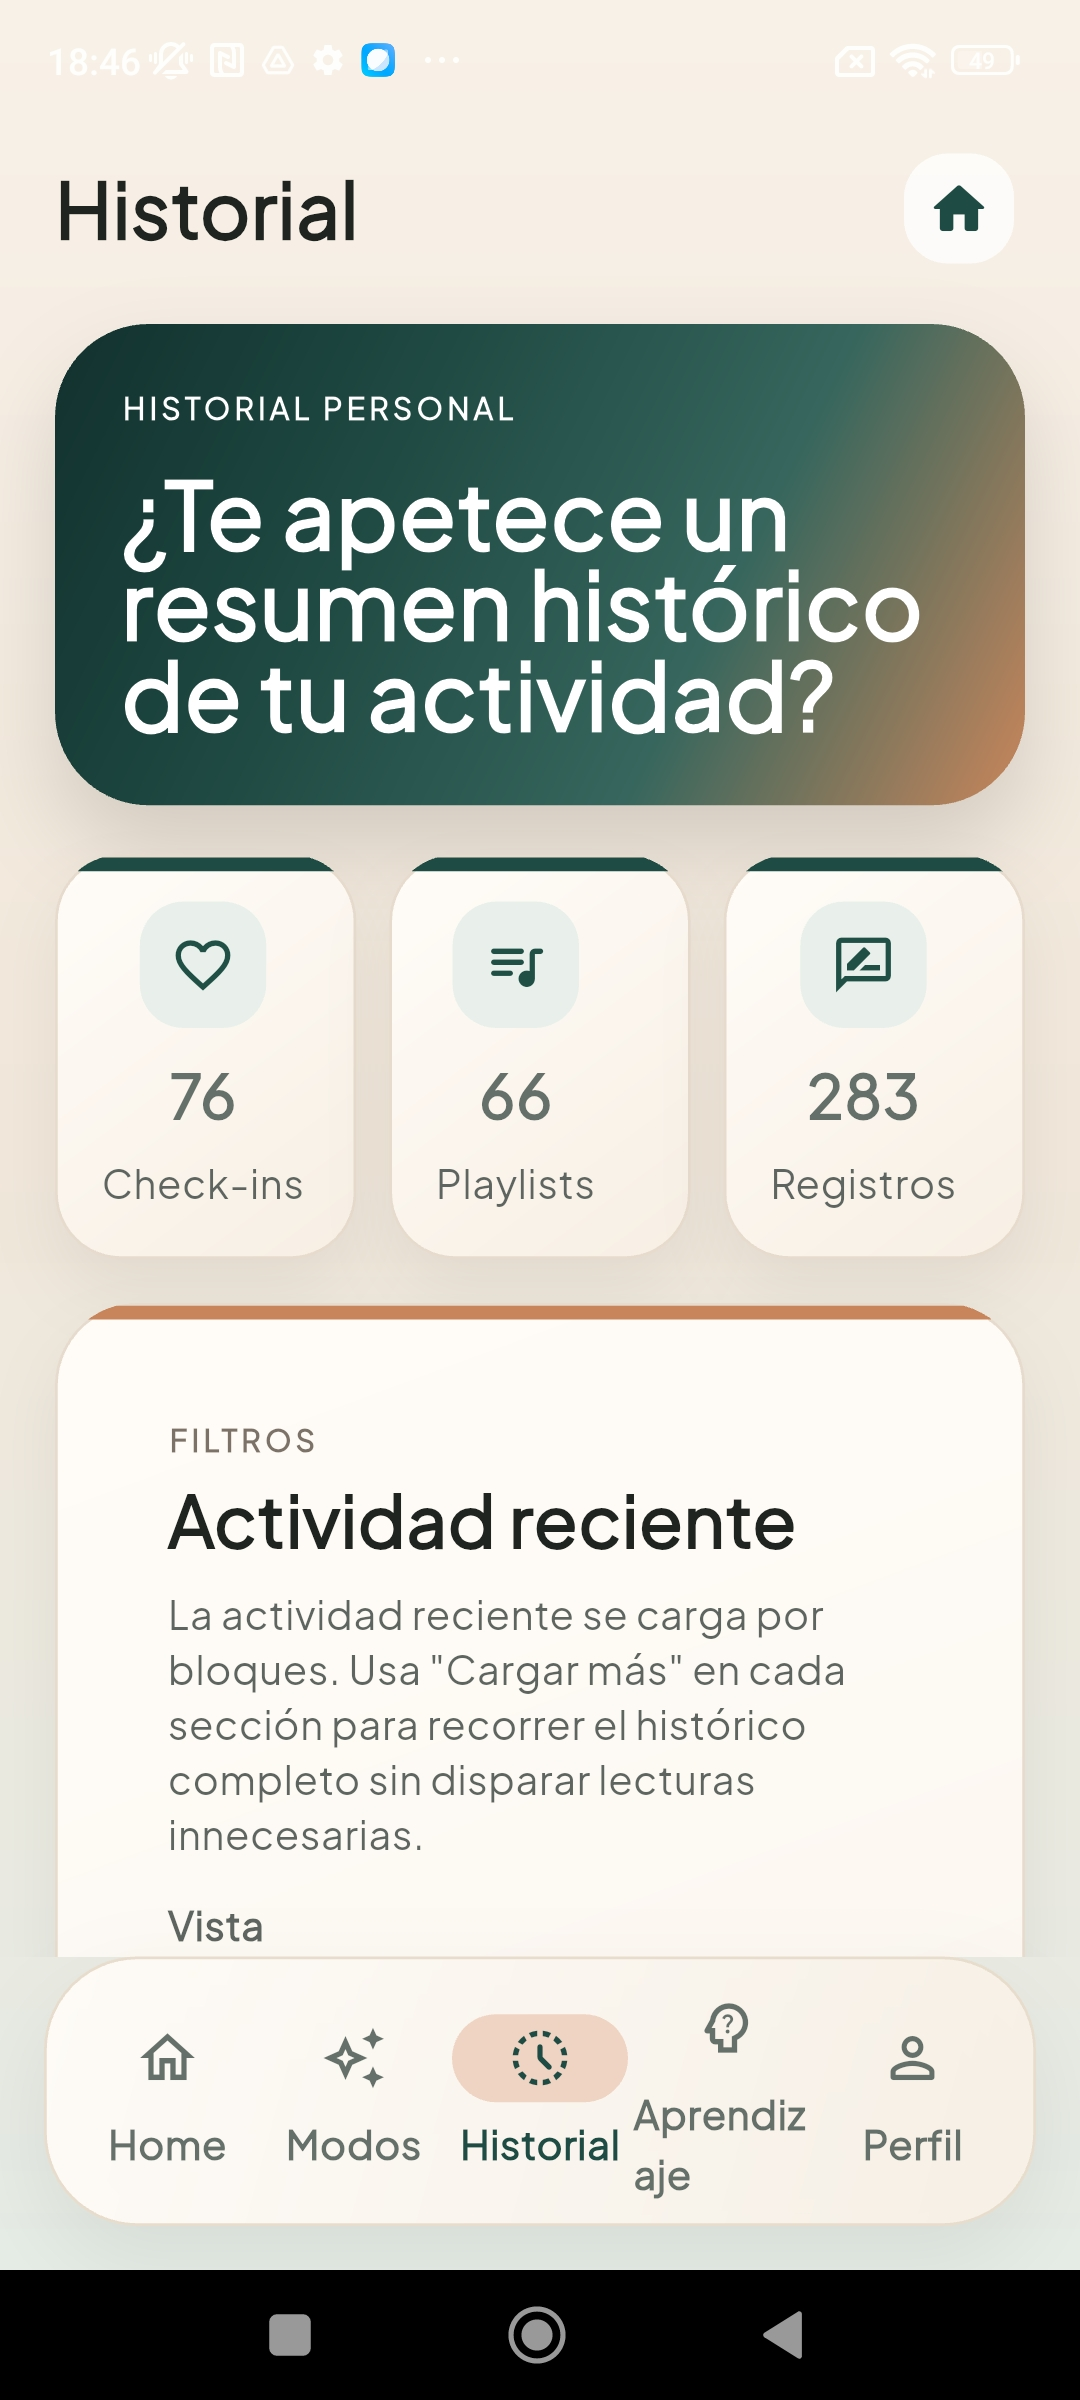
\includegraphics[width=\linewidth]{Imagenes/manual_app/Screenshot_2026-05-25-18-46-30-561_com.example.harmonyhub.jpg}
    \end{minipage}
    \hfill
    \begin{minipage}{0.47\textwidth}
        \centering
        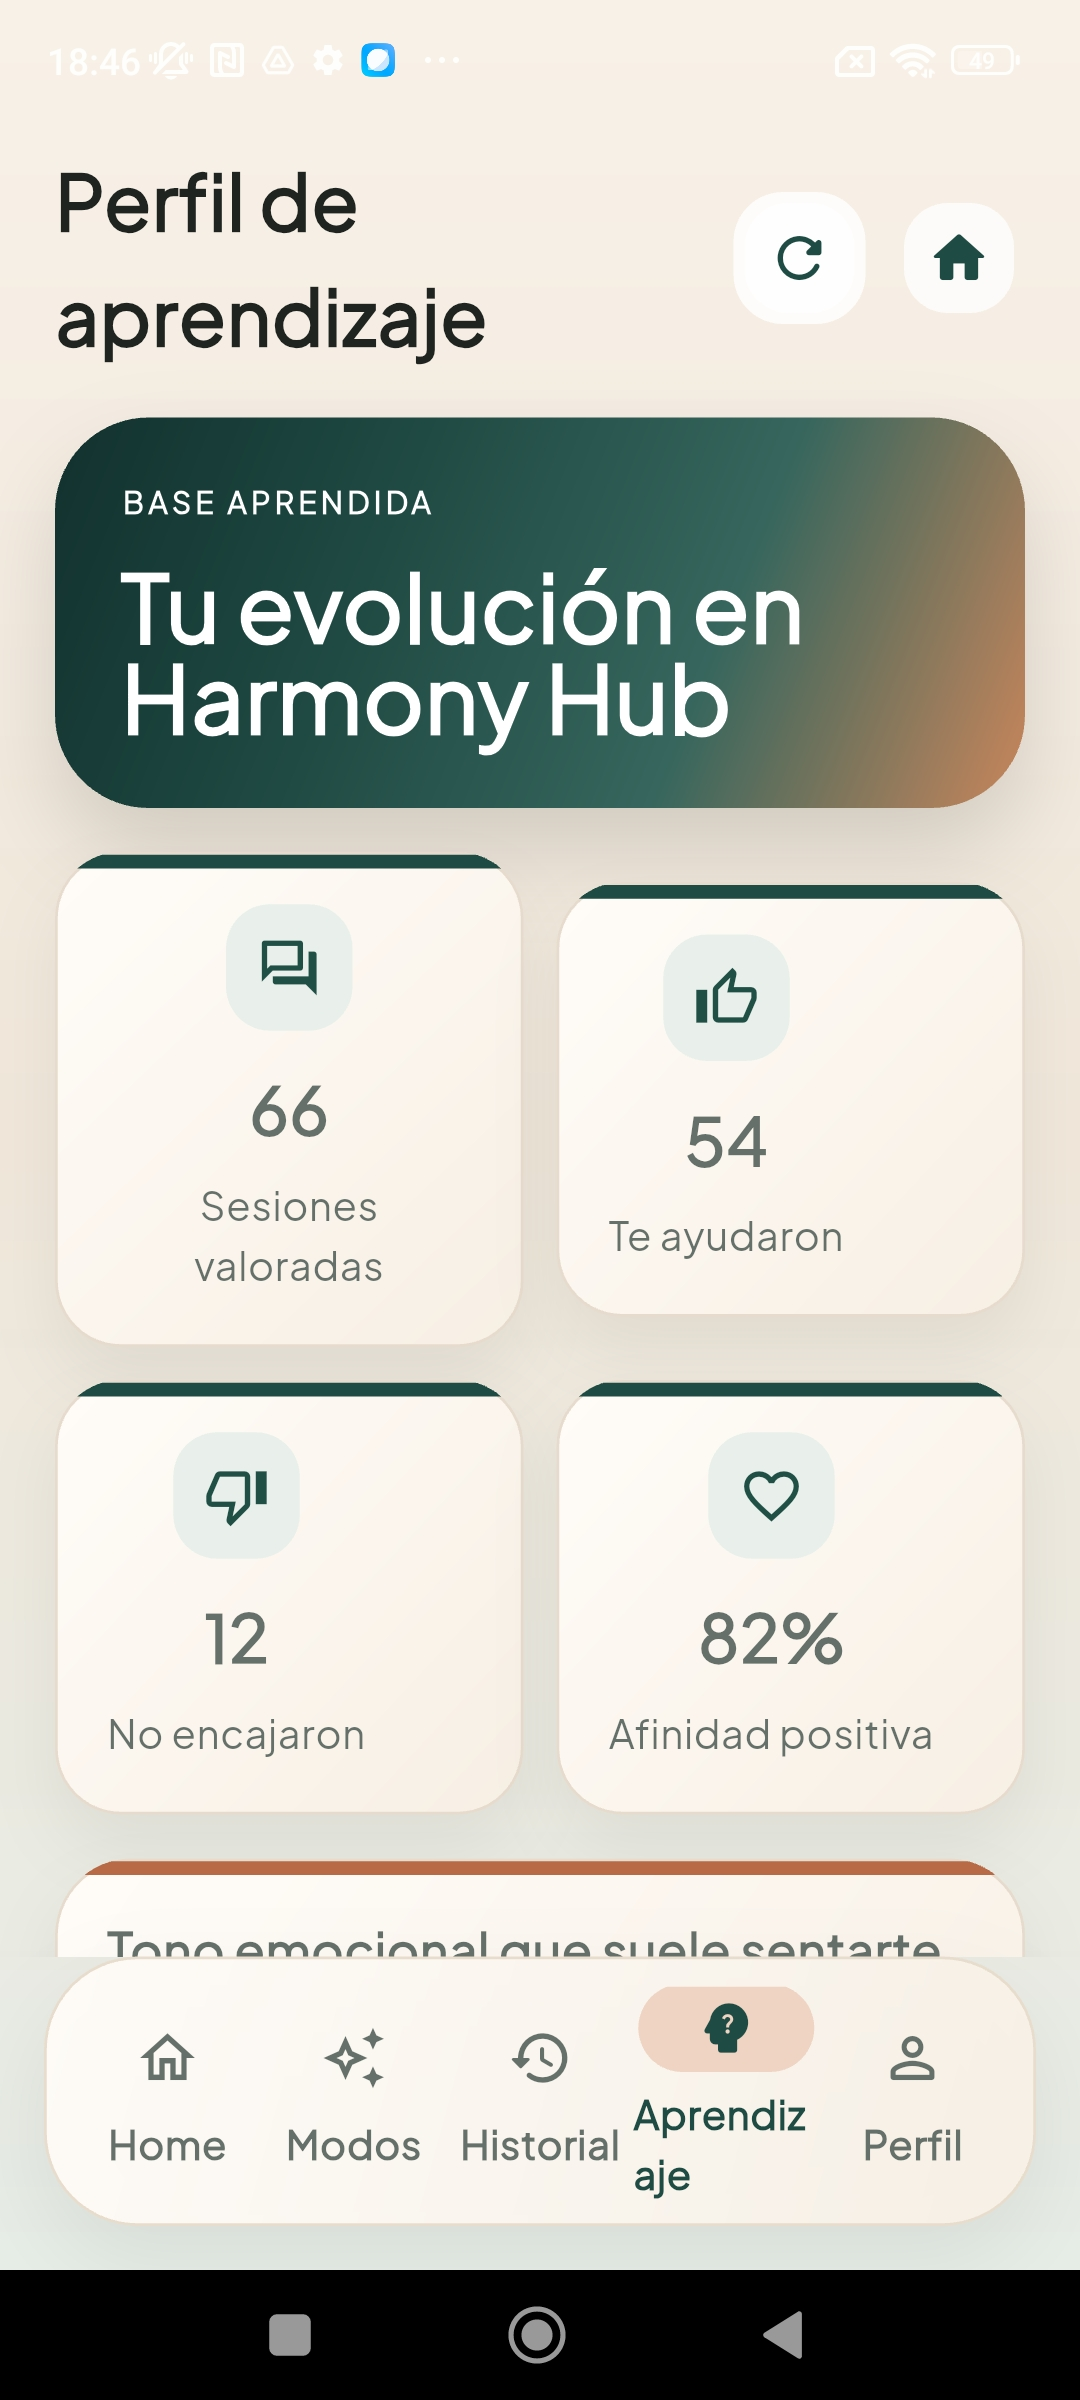
\includegraphics[width=\linewidth]{Imagenes/manual_app/Screenshot_2026-05-25-18-46-35-030_com.example.harmonyhub.jpg}
    \end{minipage}
    \caption{Bloques secundarios accesibles desde la navegación: modos
    guardados o accesos recurrentes, a la izquierda, e historial personal, a la
    derecha.}
    \label{fig:manual_modos_historial}
\end{figure}

La navegación inferior permite acceder a bloques complementarios sin romper el
flujo principal. En \textit{Modos} se muestran modos guardados, accesos rápidos
o rutas útiles para situaciones recurrentes; en \textit{Historial} se resume la
actividad previa del usuario y se facilita la revisión de sesiones ya
realizadas.

\subsection*{Aprendizaje personal}

La app muestra información resumida sobre el aprendizaje del sistema respecto a
las preferencias del usuario, incluyendo pesos contextuales y estables cuando
existe suficiente actividad acumulada.

\begin{figure}[htbp]
    \centering
    \begin{minipage}{0.31\textwidth}
        \centering
        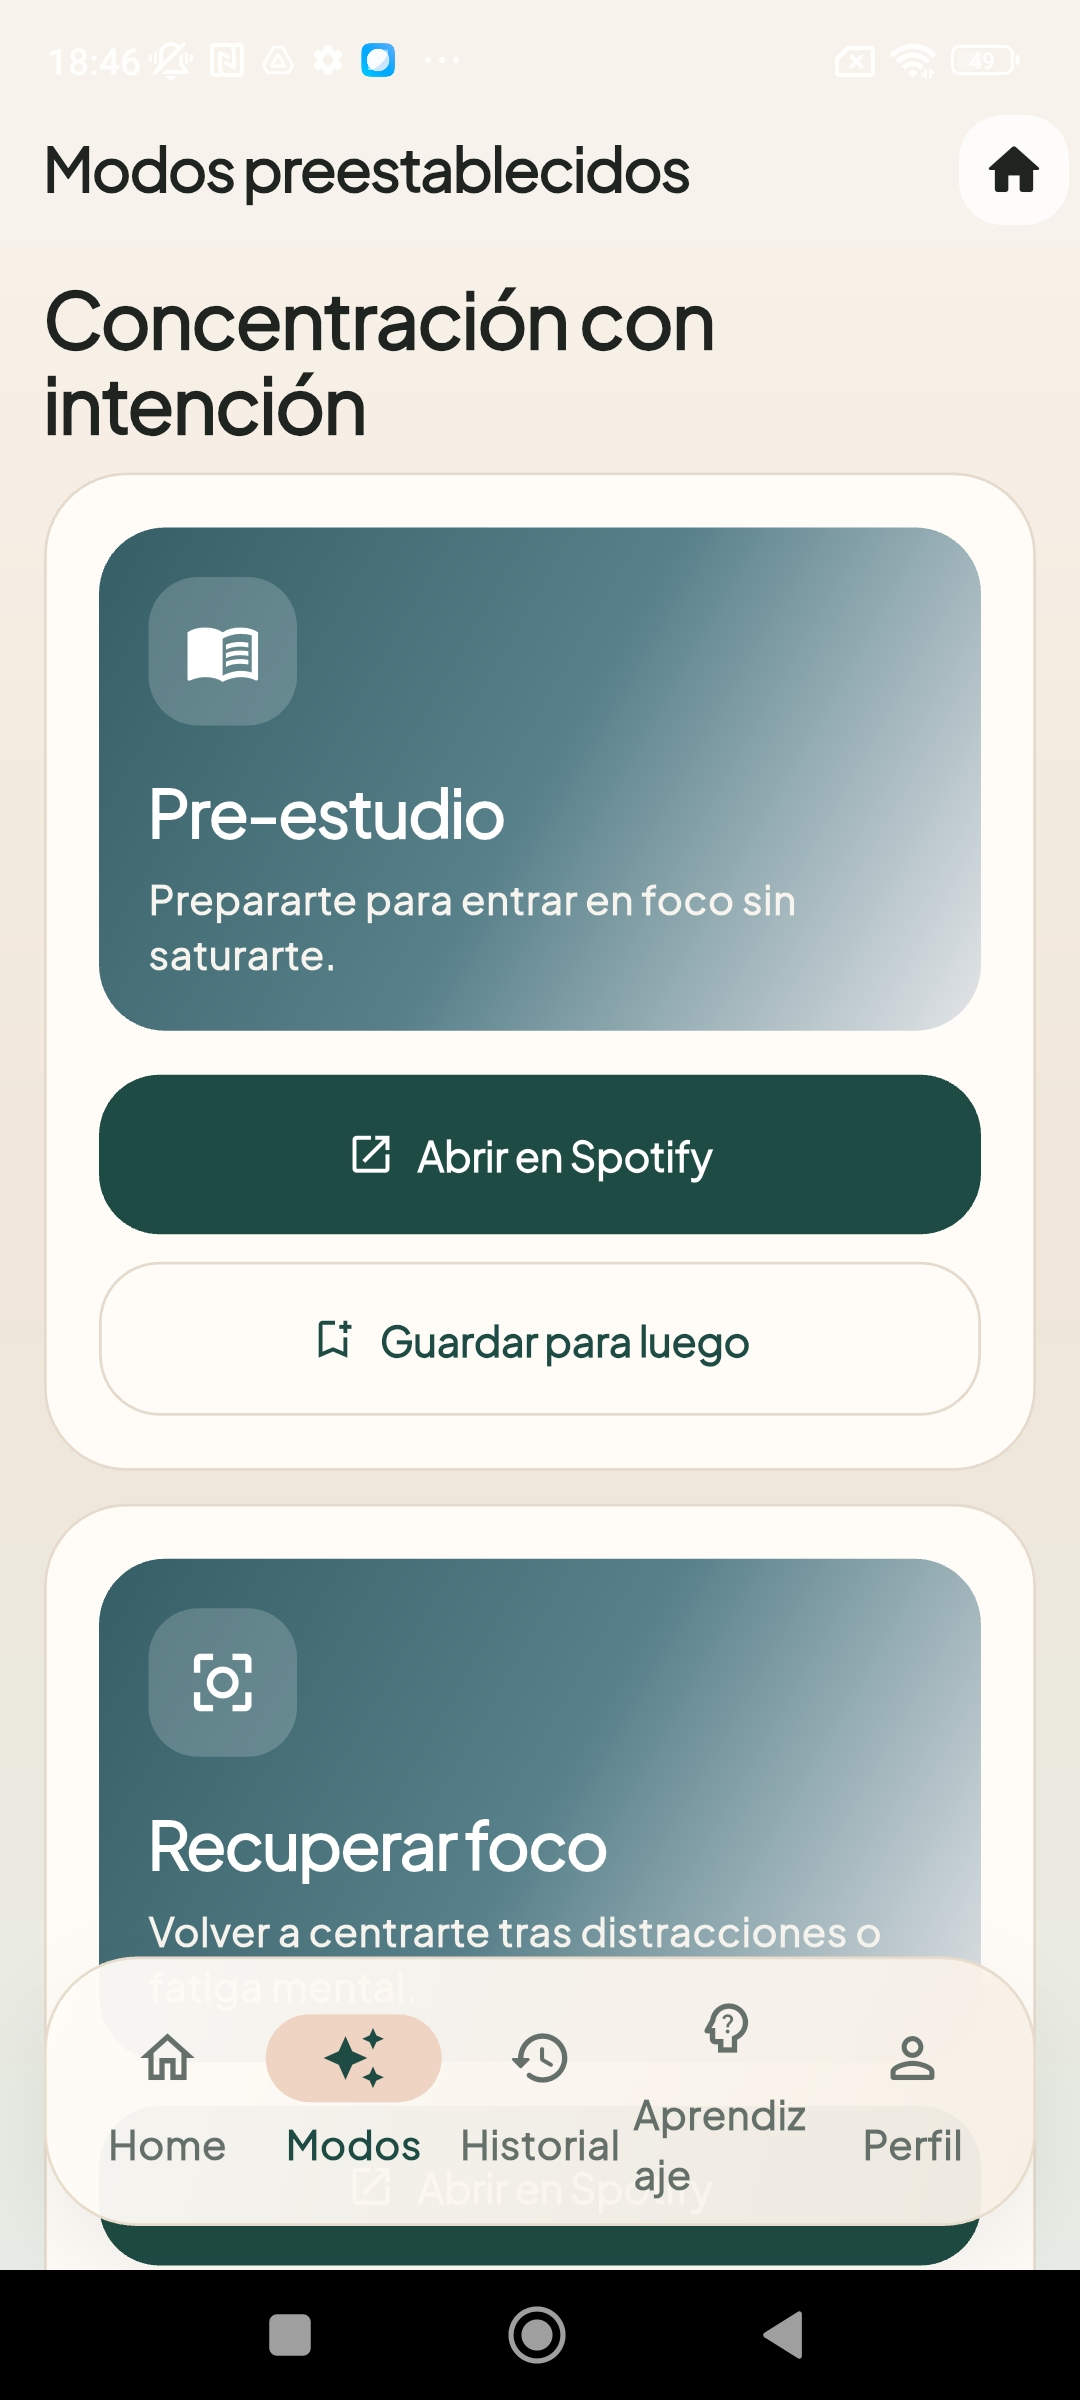
\includegraphics[width=\linewidth]{Imagenes/manual_app/Screenshot_2026-05-25-18-46-24-532_com.example.harmonyhub.jpg}
    \end{minipage}
    \hfill
    \begin{minipage}{0.31\textwidth}
        \centering
        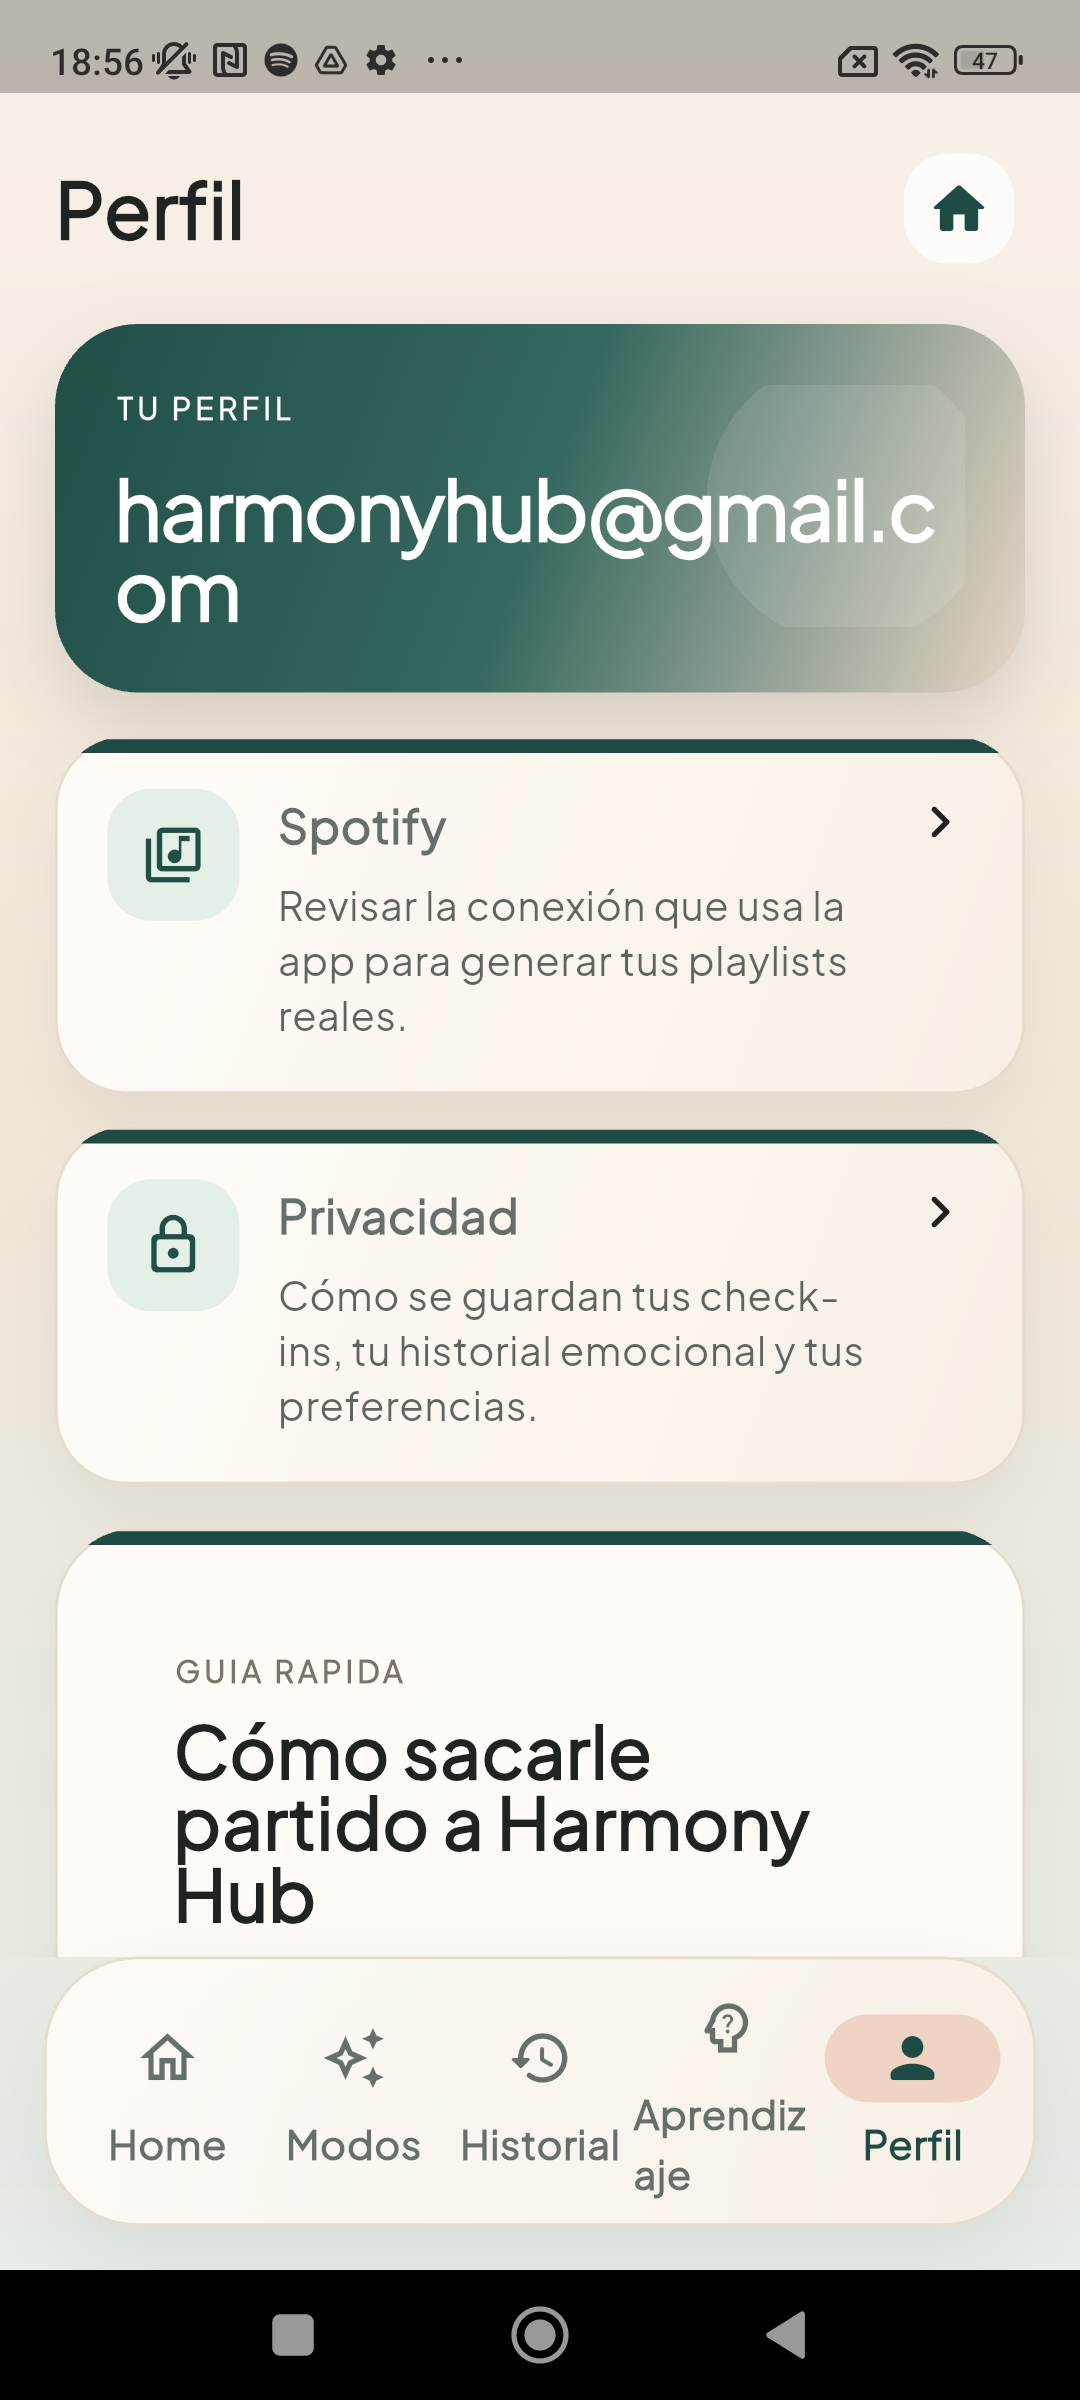
\includegraphics[width=\linewidth]{Imagenes/manual_app/Screenshot_2026-05-25-18-56-50-176_com.example.harmonyhub.jpg}
    \end{minipage}
    \hfill
    \begin{minipage}{0.31\textwidth}
        \centering
        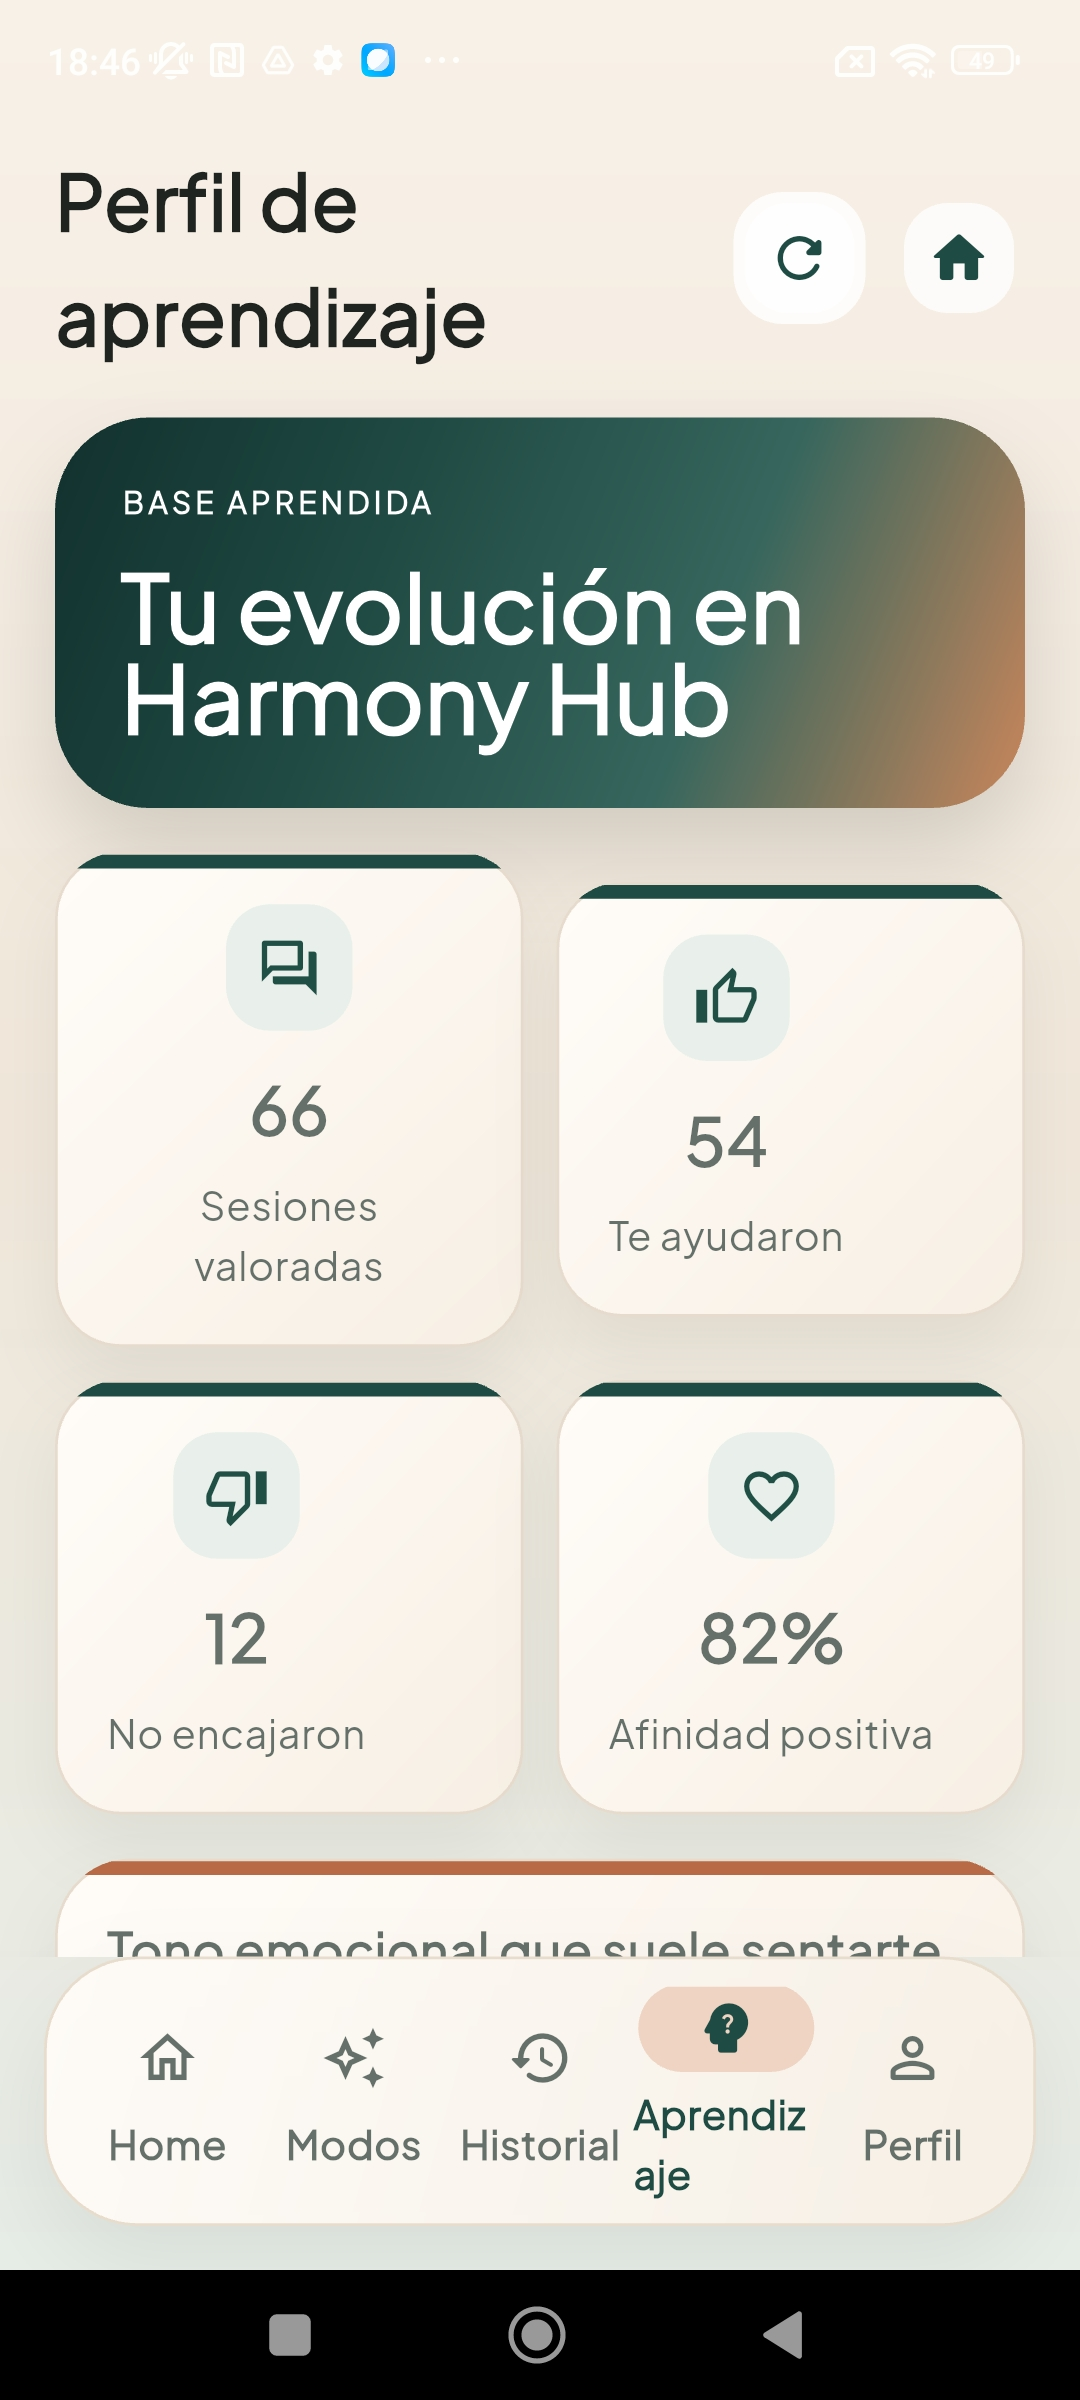
\includegraphics[width=\linewidth]{Imagenes/manual_app/Screenshot_2026-05-25-18-46-35-030_com.example.harmonyhub.jpg}
    \end{minipage}
    \caption{Pantallas de aprendizaje, perfil y modos guardados o accesos
    recurrentes entre secciones.}
    \label{fig:manual_aprendizaje_perfil}
\end{figure}

En \textit{Aprendizaje} se muestran indicadores resumidos sobre sesiones
valoradas, afinidad positiva y otras señales útiles para entender si el sistema
ya dispone de una base suficiente para personalizar mejor. En \textit{Perfil}
se agrupan opciones relacionadas con Spotify, privacidad y ayuda rápida de uso.
La tercera captura muestra el bloque de \textit{Modos}, donde aparecen modos
guardados o accesos recurrentes para reutilizar rutas funcionales frecuentes.

\subsection*{Modos guardados}

Para situaciones recurrentes, el sistema permite conservar accesos o modos
rápidos, de forma que no sea necesario repetir siempre la misma interacción
desde cero.

\section{Resolución de problemas frecuentes}
\label{sec:manual_usuario_problemas}

\subsection*{No se puede conectar Spotify}

Comprobar que:

\begin{itemize}
    \item la cuenta de Spotify ha aceptado la autorización;
    \item la redirección OAuth está bien configurada;
    \item el backend de demostración está en ejecución y accesible desde la red local;
    \item la conexión de red está disponible.
\end{itemize}

\subsection*{La recomendación se genera, pero la playlist falla}

Esto suele estar relacionado con restricciones externas de Spotify, problemas
temporales de materialización o falta de conectividad con el backend. En ese
caso conviene:

\begin{itemize}
    \item esperar unos minutos si hubo demasiadas búsquedas seguidas;
    \item volver a intentar la generación más tarde;
    \item comprobar que el móvil mantiene conectividad con la red de la demostración;
    \item comprobar que la cuenta de Spotify sigue conectada.
\end{itemize}

\subsection*{El entorno no se analiza}

Si no se ha concedido permiso de micrófono, la app seguirá funcionando, pero
sin apoyo acústico del entorno. Basta con conceder permiso cuando se quiera
utilizar esa funcionalidad.

\subsection*{No se aprecia aprendizaje todavía}

El sistema puede funcionar desde la primera sesión, pero la personalización
aprendida necesita varias sesiones cerradas con feedback. Si el usuario todavía
no ve cambios claros, conviene seguir completando sesiones y aportar feedback
útil al final de cada una.
